\documentclass[11pt,a4paper]{article}

\usepackage{geometry}
\geometry{margin=2.5cm}
\usepackage{graphicx}
\usepackage{microtype}
\usepackage{booktabs}
\usepackage{amsmath}
\usepackage{amssymb}
\usepackage[numbers,sort&compress]{natbib}
\usepackage{hyperref}
\hypersetup{hidelinks,pdfauthor={YUZHU CONG},pdftitle={Preference is not tattooability: Auditing Reward Models for AI Tattoo Generation}}
\setlength{\textfloatsep}{8pt plus 2pt minus 2pt}
\setlength{\floatsep}{8pt plus 2pt minus 2pt}
\setlength{\intextsep}{8pt plus 2pt minus 2pt}
\setlength{\abovecaptionskip}{4pt}
\setlength{\belowcaptionskip}{2pt}
\setlength{\abovedisplayskip}{6pt plus 2pt minus 2pt}
\setlength{\belowdisplayskip}{6pt plus 2pt minus 2pt}

\makeatletter
\let\paper@thebibliography\thebibliography
\renewcommand{\thebibliography}[1]{%
  \footnotesize
  \setlength{\bibsep}{0pt}%
  \enlargethispage{3\baselineskip}%
  \paper@thebibliography{#1}%
  \raggedright
}
\makeatother

% AUTO-GENERATED by tattoo-probes/scripts/make_numbers.py -- do not edit
\newcommand{\DgBorderstdfiveBlurOne}{0.50}
\newcommand{\DgBorderstdfiveBlurTwo}{0.50}
\newcommand{\DgBorderstdfiveDetaillossOne}{0.50}
\newcommand{\DgBorderstdfiveDetaillossTwo}{0.50}
\newcommand{\DgBorderstdfiveHazeOne}{1.00}
\newcommand{\DgBorderstdfiveHazeTwo}{1.00}
\newcommand{\DgBorderstdfiveSpeckleOne}{1.00}
\newcommand{\DgBorderstdfiveSpeckleTwo}{1.00}
\newcommand{\DgBorderstdfiveThickenOne}{0.50}
\newcommand{\DgBorderstdfiveThickenTwo}{0.50}
\newcommand{\DgBorderstdfiveThinOne}{0.50}
\newcommand{\DgBorderstdfiveThinTwo}{0.50}
\newcommand{\DgBorderstdtenBlurOne}{0.50}
\newcommand{\DgBorderstdtenBlurTwo}{0.50}
\newcommand{\DgBorderstdtenDetaillossOne}{0.50}
\newcommand{\DgBorderstdtenDetaillossTwo}{0.50}
\newcommand{\DgBorderstdtenHazeOne}{1.00}
\newcommand{\DgBorderstdtenHazeTwo}{1.00}
\newcommand{\DgBorderstdtenSpeckleOne}{1.00}
\newcommand{\DgBorderstdtenSpeckleTwo}{1.00}
\newcommand{\DgBorderstdtenThickenOne}{0.50}
\newcommand{\DgBorderstdtenThickenTwo}{0.50}
\newcommand{\DgBorderstdtenThinOne}{0.50}
\newcommand{\DgBorderstdtenThinTwo}{0.50}
\newcommand{\DgClipscoreBlurOne}{0.97}
\newcommand{\DgClipscoreBlurTwo}{0.70}
\newcommand{\DgClipscoreDetaillossOne}{0.77}
\newcommand{\DgClipscoreDetaillossTwo}{0.87}
\newcommand{\DgClipscoreHazeOne}{0.57}
\newcommand{\DgClipscoreHazeTwo}{0.53}
\newcommand{\DgClipscoreSpeckleOne}{0.20}
\newcommand{\DgClipscoreSpeckleTwo}{0.33}
\newcommand{\DgClipscoreThickenOne}{0.70}
\newcommand{\DgClipscoreThickenTwo}{0.63}
\newcommand{\DgClipscoreThinOne}{0.47}
\newcommand{\DgClipscoreThinTwo}{0.70}
\newcommand{\DgEdgedensitypermmfiveBlurOne}{0.03}
\newcommand{\DgEdgedensitypermmfiveBlurTwo}{0.00}
\newcommand{\DgEdgedensitypermmfiveDetaillossOne}{0.80}
\newcommand{\DgEdgedensitypermmfiveDetaillossTwo}{0.43}
\newcommand{\DgEdgedensitypermmfiveHazeOne}{1.00}
\newcommand{\DgEdgedensitypermmfiveHazeTwo}{0.60}
\newcommand{\DgEdgedensitypermmfiveSpeckleOne}{1.00}
\newcommand{\DgEdgedensitypermmfiveSpeckleTwo}{1.00}
\newcommand{\DgEdgedensitypermmfiveThickenOne}{0.07}
\newcommand{\DgEdgedensitypermmfiveThickenTwo}{0.03}
\newcommand{\DgEdgedensitypermmfiveThinOne}{0.03}
\newcommand{\DgEdgedensitypermmfiveThinTwo}{0.00}
\newcommand{\DgEdgedensitypermmtenBlurOne}{0.00}
\newcommand{\DgEdgedensitypermmtenBlurTwo}{0.00}
\newcommand{\DgEdgedensitypermmtenDetaillossOne}{0.70}
\newcommand{\DgEdgedensitypermmtenDetaillossTwo}{0.33}
\newcommand{\DgEdgedensitypermmtenHazeOne}{1.00}
\newcommand{\DgEdgedensitypermmtenHazeTwo}{1.00}
\newcommand{\DgEdgedensitypermmtenSpeckleOne}{1.00}
\newcommand{\DgEdgedensitypermmtenSpeckleTwo}{1.00}
\newcommand{\DgEdgedensitypermmtenThickenOne}{0.07}
\newcommand{\DgEdgedensitypermmtenThickenTwo}{0.00}
\newcommand{\DgEdgedensitypermmtenThinOne}{0.07}
\newcommand{\DgEdgedensitypermmtenThinTwo}{0.03}
\newcommand{\DgEdgetransitionmmfiveBlurOne}{0.97}
\newcommand{\DgEdgetransitionmmfiveBlurTwo}{0.97}
\newcommand{\DgEdgetransitionmmfiveDetaillossOne}{1.00}
\newcommand{\DgEdgetransitionmmfiveDetaillossTwo}{0.97}
\newcommand{\DgEdgetransitionmmfiveHazeOne}{0.47}
\newcommand{\DgEdgetransitionmmfiveHazeTwo}{0.23}
\newcommand{\DgEdgetransitionmmfiveSpeckleOne}{0.73}
\newcommand{\DgEdgetransitionmmfiveSpeckleTwo}{0.73}
\newcommand{\DgEdgetransitionmmfiveThickenOne}{0.90}
\newcommand{\DgEdgetransitionmmfiveThickenTwo}{1.00}
\newcommand{\DgEdgetransitionmmfiveThinOne}{0.83}
\newcommand{\DgEdgetransitionmmfiveThinTwo}{0.83}
\newcommand{\DgEdgetransitionmmtenBlurOne}{0.93}
\newcommand{\DgEdgetransitionmmtenBlurTwo}{0.63}
\newcommand{\DgEdgetransitionmmtenDetaillossOne}{0.93}
\newcommand{\DgEdgetransitionmmtenDetaillossTwo}{0.90}
\newcommand{\DgEdgetransitionmmtenHazeOne}{1.00}
\newcommand{\DgEdgetransitionmmtenHazeTwo}{0.97}
\newcommand{\DgEdgetransitionmmtenSpeckleOne}{0.00}
\newcommand{\DgEdgetransitionmmtenSpeckleTwo}{0.00}
\newcommand{\DgEdgetransitionmmtenThickenOne}{0.97}
\newcommand{\DgEdgetransitionmmtenThickenTwo}{0.97}
\newcommand{\DgEdgetransitionmmtenThinOne}{0.70}
\newcommand{\DgEdgetransitionmmtenThinTwo}{0.77}
\newcommand{\DgFracsubneedlefiveBlurOne}{0.00}
\newcommand{\DgFracsubneedlefiveBlurTwo}{0.00}
\newcommand{\DgFracsubneedlefiveDetaillossOne}{0.13}
\newcommand{\DgFracsubneedlefiveDetaillossTwo}{0.13}
\newcommand{\DgFracsubneedlefiveHazeOne}{0.83}
\newcommand{\DgFracsubneedlefiveHazeTwo}{0.97}
\newcommand{\DgFracsubneedlefiveSpeckleOne}{1.00}
\newcommand{\DgFracsubneedlefiveSpeckleTwo}{1.00}
\newcommand{\DgFracsubneedlefiveThickenOne}{0.10}
\newcommand{\DgFracsubneedlefiveThickenTwo}{0.03}
\newcommand{\DgFracsubneedlefiveThinOne}{0.50}
\newcommand{\DgFracsubneedlefiveThinTwo}{0.43}
\newcommand{\DgFracsubneedletenBlurOne}{0.10}
\newcommand{\DgFracsubneedletenBlurTwo}{0.03}
\newcommand{\DgFracsubneedletenDetaillossOne}{0.67}
\newcommand{\DgFracsubneedletenDetaillossTwo}{0.57}
\newcommand{\DgFracsubneedletenHazeOne}{0.90}
\newcommand{\DgFracsubneedletenHazeTwo}{0.93}
\newcommand{\DgFracsubneedletenSpeckleOne}{1.00}
\newcommand{\DgFracsubneedletenSpeckleTwo}{1.00}
\newcommand{\DgFracsubneedletenThickenOne}{0.23}
\newcommand{\DgFracsubneedletenThickenTwo}{0.10}
\newcommand{\DgFracsubneedletenThinOne}{0.70}
\newcommand{\DgFracsubneedletenThinTwo}{0.67}
\newcommand{\DgFractightgapfiveBlurOne}{0.10}
\newcommand{\DgFractightgapfiveBlurTwo}{0.00}
\newcommand{\DgFractightgapfiveDetaillossOne}{0.20}
\newcommand{\DgFractightgapfiveDetaillossTwo}{0.03}
\newcommand{\DgFractightgapfiveHazeOne}{0.97}
\newcommand{\DgFractightgapfiveHazeTwo}{0.93}
\newcommand{\DgFractightgapfiveSpeckleOne}{0.33}
\newcommand{\DgFractightgapfiveSpeckleTwo}{0.70}
\newcommand{\DgFractightgapfiveThickenOne}{0.37}
\newcommand{\DgFractightgapfiveThickenTwo}{0.37}
\newcommand{\DgFractightgapfiveThinOne}{0.07}
\newcommand{\DgFractightgapfiveThinTwo}{0.07}
\newcommand{\DgFractightgaptenBlurOne}{0.07}
\newcommand{\DgFractightgaptenBlurTwo}{0.10}
\newcommand{\DgFractightgaptenDetaillossOne}{0.50}
\newcommand{\DgFractightgaptenDetaillossTwo}{0.47}
\newcommand{\DgFractightgaptenHazeOne}{0.87}
\newcommand{\DgFractightgaptenHazeTwo}{0.97}
\newcommand{\DgFractightgaptenSpeckleOne}{0.03}
\newcommand{\DgFractightgaptenSpeckleTwo}{0.10}
\newcommand{\DgFractightgaptenThickenOne}{0.53}
\newcommand{\DgFractightgaptenThickenTwo}{0.47}
\newcommand{\DgFractightgaptenThinOne}{0.07}
\newcommand{\DgFractightgaptenThinTwo}{0.07}
\newcommand{\DgHpstwoBlurOne}{0.80}
\newcommand{\DgHpstwoBlurTwo}{0.97}
\newcommand{\DgHpstwoDetaillossOne}{0.97}
\newcommand{\DgHpstwoDetaillossTwo}{1.00}
\newcommand{\DgHpstwoHazeOne}{1.00}
\newcommand{\DgHpstwoHazeTwo}{1.00}
\newcommand{\DgHpstwoSpeckleOne}{1.00}
\newcommand{\DgHpstwoSpeckleTwo}{1.00}
\newcommand{\DgHpstwoThickenOne}{0.87}
\newcommand{\DgHpstwoThickenTwo}{0.97}
\newcommand{\DgHpstwoThinOne}{0.90}
\newcommand{\DgHpstwoThinTwo}{1.00}
\newcommand{\DgImagerewardBlurOne}{0.90}
\newcommand{\DgImagerewardBlurTwo}{0.90}
\newcommand{\DgImagerewardDetaillossOne}{0.87}
\newcommand{\DgImagerewardDetaillossTwo}{0.93}
\newcommand{\DgImagerewardHazeOne}{0.77}
\newcommand{\DgImagerewardHazeTwo}{0.83}
\newcommand{\DgImagerewardSpeckleOne}{0.60}
\newcommand{\DgImagerewardSpeckleTwo}{0.47}
\newcommand{\DgImagerewardThickenOne}{0.77}
\newcommand{\DgImagerewardThickenTwo}{0.87}
\newcommand{\DgImagerewardThinOne}{0.83}
\newcommand{\DgImagerewardThinTwo}{0.90}
\newcommand{\DgLinewpmmfiveBlurOne}{0.07}
\newcommand{\DgLinewpmmfiveBlurTwo}{0.03}
\newcommand{\DgLinewpmmfiveDetaillossOne}{0.18}
\newcommand{\DgLinewpmmfiveDetaillossTwo}{0.02}
\newcommand{\DgLinewpmmfiveHazeOne}{0.67}
\newcommand{\DgLinewpmmfiveHazeTwo}{0.68}
\newcommand{\DgLinewpmmfiveSpeckleOne}{0.78}
\newcommand{\DgLinewpmmfiveSpeckleTwo}{0.78}
\newcommand{\DgLinewpmmfiveThickenOne}{0.02}
\newcommand{\DgLinewpmmfiveThickenTwo}{0.00}
\newcommand{\DgLinewpmmfiveThinOne}{0.65}
\newcommand{\DgLinewpmmfiveThinTwo}{0.57}
\newcommand{\DgLinewpmmtenBlurOne}{0.02}
\newcommand{\DgLinewpmmtenBlurTwo}{0.03}
\newcommand{\DgLinewpmmtenDetaillossOne}{0.67}
\newcommand{\DgLinewpmmtenDetaillossTwo}{0.37}
\newcommand{\DgLinewpmmtenHazeOne}{0.77}
\newcommand{\DgLinewpmmtenHazeTwo}{0.77}
\newcommand{\DgLinewpmmtenSpeckleOne}{0.92}
\newcommand{\DgLinewpmmtenSpeckleTwo}{0.92}
\newcommand{\DgLinewpmmtenThickenOne}{0.05}
\newcommand{\DgLinewpmmtenThickenTwo}{0.00}
\newcommand{\DgLinewpmmtenThinOne}{0.72}
\newcommand{\DgLinewpmmtenThinTwo}{0.70}
\newcommand{\DgMidtonefracfiveBlurOne}{0.93}
\newcommand{\DgMidtonefracfiveBlurTwo}{0.93}
\newcommand{\DgMidtonefracfiveDetaillossOne}{0.97}
\newcommand{\DgMidtonefracfiveDetaillossTwo}{0.93}
\newcommand{\DgMidtonefracfiveHazeOne}{1.00}
\newcommand{\DgMidtonefracfiveHazeTwo}{1.00}
\newcommand{\DgMidtonefracfiveSpeckleOne}{1.00}
\newcommand{\DgMidtonefracfiveSpeckleTwo}{1.00}
\newcommand{\DgMidtonefracfiveThickenOne}{0.43}
\newcommand{\DgMidtonefracfiveThickenTwo}{0.33}
\newcommand{\DgMidtonefracfiveThinOne}{0.33}
\newcommand{\DgMidtonefracfiveThinTwo}{0.20}
\newcommand{\DgMidtonefractenBlurOne}{0.93}
\newcommand{\DgMidtonefractenBlurTwo}{0.93}
\newcommand{\DgMidtonefractenDetaillossOne}{0.97}
\newcommand{\DgMidtonefractenDetaillossTwo}{0.93}
\newcommand{\DgMidtonefractenHazeOne}{1.00}
\newcommand{\DgMidtonefractenHazeTwo}{1.00}
\newcommand{\DgMidtonefractenSpeckleOne}{1.00}
\newcommand{\DgMidtonefractenSpeckleTwo}{1.00}
\newcommand{\DgMidtonefractenThickenOne}{0.43}
\newcommand{\DgMidtonefractenThickenTwo}{0.37}
\newcommand{\DgMidtonefractenThinOne}{0.33}
\newcommand{\DgMidtonefractenThinTwo}{0.23}
\newcommand{\DgOpenendspercmfiveBlurOne}{0.13}
\newcommand{\DgOpenendspercmfiveBlurTwo}{0.27}
\newcommand{\DgOpenendspercmfiveDetaillossOne}{0.43}
\newcommand{\DgOpenendspercmfiveDetaillossTwo}{0.27}
\newcommand{\DgOpenendspercmfiveHazeOne}{0.73}
\newcommand{\DgOpenendspercmfiveHazeTwo}{0.73}
\newcommand{\DgOpenendspercmfiveSpeckleOne}{1.00}
\newcommand{\DgOpenendspercmfiveSpeckleTwo}{1.00}
\newcommand{\DgOpenendspercmfiveThickenOne}{0.20}
\newcommand{\DgOpenendspercmfiveThickenTwo}{0.23}
\newcommand{\DgOpenendspercmfiveThinOne}{0.77}
\newcommand{\DgOpenendspercmfiveThinTwo}{0.83}
\newcommand{\DgOpenendspercmtenBlurOne}{0.10}
\newcommand{\DgOpenendspercmtenBlurTwo}{0.20}
\newcommand{\DgOpenendspercmtenDetaillossOne}{0.90}
\newcommand{\DgOpenendspercmtenDetaillossTwo}{0.53}
\newcommand{\DgOpenendspercmtenHazeOne}{0.77}
\newcommand{\DgOpenendspercmtenHazeTwo}{0.90}
\newcommand{\DgOpenendspercmtenSpeckleOne}{1.00}
\newcommand{\DgOpenendspercmtenSpeckleTwo}{1.00}
\newcommand{\DgOpenendspercmtenThickenOne}{0.20}
\newcommand{\DgOpenendspercmtenThickenTwo}{0.17}
\newcommand{\DgOpenendspercmtenThinOne}{0.80}
\newcommand{\DgOpenendspercmtenThinTwo}{0.80}
\newcommand{\DgPickscoreBlurOne}{0.53}
\newcommand{\DgPickscoreBlurTwo}{0.87}
\newcommand{\DgPickscoreDetaillossOne}{0.83}
\newcommand{\DgPickscoreDetaillossTwo}{0.97}
\newcommand{\DgPickscoreHazeOne}{0.80}
\newcommand{\DgPickscoreHazeTwo}{0.97}
\newcommand{\DgPickscoreSpeckleOne}{0.70}
\newcommand{\DgPickscoreSpeckleTwo}{0.83}
\newcommand{\DgPickscoreThickenOne}{0.97}
\newcommand{\DgPickscoreThickenTwo}{0.97}
\newcommand{\DgPickscoreThinOne}{0.97}
\newcommand{\DgPickscoreThinTwo}{1.00}
\newcommand{\DgProbecompositefiveBlurOne}{0.27}
\newcommand{\DgProbecompositefiveBlurTwo}{0.23}
\newcommand{\DgProbecompositefiveDetaillossOne}{0.53}
\newcommand{\DgProbecompositefiveDetaillossTwo}{0.20}
\newcommand{\DgProbecompositefiveHazeOne}{1.00}
\newcommand{\DgProbecompositefiveHazeTwo}{1.00}
\newcommand{\DgProbecompositefiveSpeckleOne}{1.00}
\newcommand{\DgProbecompositefiveSpeckleTwo}{1.00}
\newcommand{\DgProbecompositefiveThickenOne}{0.00}
\newcommand{\DgProbecompositefiveThickenTwo}{0.00}
\newcommand{\DgProbecompositefiveThinOne}{0.57}
\newcommand{\DgProbecompositefiveThinTwo}{0.43}
\newcommand{\DgProbecompositetenBlurOne}{0.30}
\newcommand{\DgProbecompositetenBlurTwo}{0.10}
\newcommand{\DgProbecompositetenDetaillossOne}{0.73}
\newcommand{\DgProbecompositetenDetaillossTwo}{0.57}
\newcommand{\DgProbecompositetenHazeOne}{1.00}
\newcommand{\DgProbecompositetenHazeTwo}{1.00}
\newcommand{\DgProbecompositetenSpeckleOne}{1.00}
\newcommand{\DgProbecompositetenSpeckleTwo}{1.00}
\newcommand{\DgProbecompositetenThickenOne}{0.07}
\newcommand{\DgProbecompositetenThickenTwo}{0.03}
\newcommand{\DgProbecompositetenThinOne}{0.53}
\newcommand{\DgProbecompositetenThinTwo}{0.50}
\newcommand{\DgSpeckspercmfiveBlurOne}{0.20}
\newcommand{\DgSpeckspercmfiveBlurTwo}{0.20}
\newcommand{\DgSpeckspercmfiveDetaillossOne}{0.18}
\newcommand{\DgSpeckspercmfiveDetaillossTwo}{0.18}
\newcommand{\DgSpeckspercmfiveHazeOne}{0.87}
\newcommand{\DgSpeckspercmfiveHazeTwo}{0.92}
\newcommand{\DgSpeckspercmfiveSpeckleOne}{1.00}
\newcommand{\DgSpeckspercmfiveSpeckleTwo}{1.00}
\newcommand{\DgSpeckspercmfiveThickenOne}{0.22}
\newcommand{\DgSpeckspercmfiveThickenTwo}{0.18}
\newcommand{\DgSpeckspercmfiveThinOne}{0.65}
\newcommand{\DgSpeckspercmfiveThinTwo}{0.65}
\newcommand{\DgSpeckspercmtenBlurOne}{0.25}
\newcommand{\DgSpeckspercmtenBlurTwo}{0.23}
\newcommand{\DgSpeckspercmtenDetaillossOne}{0.90}
\newcommand{\DgSpeckspercmtenDetaillossTwo}{0.55}
\newcommand{\DgSpeckspercmtenHazeOne}{0.87}
\newcommand{\DgSpeckspercmtenHazeTwo}{0.92}
\newcommand{\DgSpeckspercmtenSpeckleOne}{1.00}
\newcommand{\DgSpeckspercmtenSpeckleTwo}{1.00}
\newcommand{\DgSpeckspercmtenThickenOne}{0.30}
\newcommand{\DgSpeckspercmtenThickenTwo}{0.27}
\newcommand{\DgSpeckspercmtenThinOne}{0.75}
\newcommand{\DgSpeckspercmtenThinTwo}{0.65}
\newcommand{\FusHpdProbesallAcc}{0.701}
\newcommand{\FusHpdProbesallHi}{0.745}
\newcommand{\FusHpdProbesallLo}{0.656}
\newcommand{\FusHpdProbesallN}{528}
\newcommand{\FusHpdProbespreregisteredAcc}{0.708}
\newcommand{\FusHpdProbespreregisteredHi}{0.750}
\newcommand{\FusHpdProbespreregisteredLo}{0.667}
\newcommand{\FusHpdProbespreregisteredN}{528}
\newcommand{\FusHpdRewardsAcc}{0.790}
\newcommand{\FusHpdRewardsHi}{0.827}
\newcommand{\FusHpdRewardsLo}{0.748}
\newcommand{\FusHpdRewardsN}{528}
\newcommand{\FusHpdRewardsprobesAcc}{0.767}
\newcommand{\FusHpdRewardsprobesHi}{0.803}
\newcommand{\FusHpdRewardsprobesLo}{0.729}
\newcommand{\FusHpdRewardsprobesN}{528}
\newcommand{\FusIrProbesallAcc}{0.480}
\newcommand{\FusIrProbesallHi}{0.695}
\newcommand{\FusIrProbesallLo}{0.308}
\newcommand{\FusIrProbesallN}{148}
\newcommand{\FusIrProbespreregisteredAcc}{0.500}
\newcommand{\FusIrProbespreregisteredHi}{0.702}
\newcommand{\FusIrProbespreregisteredLo}{0.329}
\newcommand{\FusIrProbespreregisteredN}{148}
\newcommand{\FusIrRewardsAcc}{0.662}
\newcommand{\FusIrRewardsHi}{0.767}
\newcommand{\FusIrRewardsLo}{0.545}
\newcommand{\FusIrRewardsN}{148}
\newcommand{\FusIrRewardsprobesAcc}{0.561}
\newcommand{\FusIrRewardsprobesHi}{0.724}
\newcommand{\FusIrRewardsprobesLo}{0.403}
\newcommand{\FusIrRewardsprobesN}{148}
\newcommand{\FusPapProbesallAcc}{0.385}
\newcommand{\FusPapProbesallHi}{0.711}
\newcommand{\FusPapProbesallLo}{0.252}
\newcommand{\FusPapProbesallN}{65}
\newcommand{\FusPapProbespreregisteredAcc}{0.400}
\newcommand{\FusPapProbespreregisteredHi}{0.757}
\newcommand{\FusPapProbespreregisteredLo}{0.266}
\newcommand{\FusPapProbespreregisteredN}{65}
\newcommand{\FusPapRewardsAcc}{0.831}
\newcommand{\FusPapRewardsHi}{0.939}
\newcommand{\FusPapRewardsLo}{0.687}
\newcommand{\FusPapRewardsN}{65}
\newcommand{\FusPapRewardsprobesAcc}{0.785}
\newcommand{\FusPapRewardsprobesHi}{0.896}
\newcommand{\FusPapRewardsprobesLo}{0.700}
\newcommand{\FusPapRewardsprobesN}{65}
\newcommand{\HpdBorderstdfiveAcc}{0.377}
\newcommand{\HpdBorderstdfiveEffect}{-0.123}
\newcommand{\HpdBorderstdfiveH}{-0.25}
\newcommand{\HpdBorderstdfiveHi}{0.425}
\newcommand{\HpdBorderstdfiveLo}{0.332}
\newcommand{\HpdBorderstdfiveN}{528}
\newcommand{\HpdBorderstdfivePholm}{0.006}
\newcommand{\HpdClipscoreAcc}{0.682}
\newcommand{\HpdClipscoreEffect}{+0.182}
\newcommand{\HpdClipscoreH}{+0.37}
\newcommand{\HpdClipscoreHi}{0.724}
\newcommand{\HpdClipscoreLo}{0.635}
\newcommand{\HpdClipscoreN}{528}
\newcommand{\HpdClipscorePholm}{0.006}
\newcommand{\HpdEdgedensitypermmfiveAcc}{0.335}
\newcommand{\HpdEdgedensitypermmfiveEffect}{-0.165}
\newcommand{\HpdEdgedensitypermmfiveH}{-0.34}
\newcommand{\HpdEdgedensitypermmfiveHi}{0.380}
\newcommand{\HpdEdgedensitypermmfiveLo}{0.295}
\newcommand{\HpdEdgedensitypermmfiveN}{528}
\newcommand{\HpdEdgedensitypermmfivePholm}{0.006}
\newcommand{\HpdEdgetransitionmmfiveAcc}{0.460}
\newcommand{\HpdEdgetransitionmmfiveEffect}{-0.040}
\newcommand{\HpdEdgetransitionmmfiveH}{-0.08}
\newcommand{\HpdEdgetransitionmmfiveHi}{0.513}
\newcommand{\HpdEdgetransitionmmfiveLo}{0.408}
\newcommand{\HpdEdgetransitionmmfiveN}{528}
\newcommand{\HpdEdgetransitionmmfivePholm}{0.279}
\newcommand{\HpdFracsubneedlefiveAcc}{0.411}
\newcommand{\HpdFracsubneedlefiveEffect}{-0.089}
\newcommand{\HpdFracsubneedlefiveH}{-0.18}
\newcommand{\HpdFracsubneedlefiveHi}{0.462}
\newcommand{\HpdFracsubneedlefiveLo}{0.361}
\newcommand{\HpdFracsubneedlefiveN}{528}
\newcommand{\HpdFracsubneedlefivePholm}{0.006}
\newcommand{\HpdFractightgapfiveAcc}{0.335}
\newcommand{\HpdFractightgapfiveEffect}{-0.165}
\newcommand{\HpdFractightgapfiveH}{-0.34}
\newcommand{\HpdFractightgapfiveHi}{0.383}
\newcommand{\HpdFractightgapfiveLo}{0.288}
\newcommand{\HpdFractightgapfiveN}{528}
\newcommand{\HpdFractightgapfivePholm}{0.006}
\newcommand{\HpdHpstwoAcc}{0.790}
\newcommand{\HpdHpstwoEffect}{+0.290}
\newcommand{\HpdHpstwoH}{+0.62}
\newcommand{\HpdHpstwoHi}{0.827}
\newcommand{\HpdHpstwoLo}{0.751}
\newcommand{\HpdHpstwoN}{528}
\newcommand{\HpdHpstwoPholm}{0.006}
\newcommand{\HpdImagerewardAcc}{0.684}
\newcommand{\HpdImagerewardEffect}{+0.184}
\newcommand{\HpdImagerewardH}{+0.38}
\newcommand{\HpdImagerewardHi}{0.730}
\newcommand{\HpdImagerewardLo}{0.634}
\newcommand{\HpdImagerewardN}{528}
\newcommand{\HpdImagerewardPholm}{0.006}
\newcommand{\HpdLinewpmmfiveAcc}{0.428}
\newcommand{\HpdLinewpmmfiveEffect}{-0.072}
\newcommand{\HpdLinewpmmfiveH}{-0.14}
\newcommand{\HpdLinewpmmfiveHi}{0.458}
\newcommand{\HpdLinewpmmfiveLo}{0.399}
\newcommand{\HpdLinewpmmfiveN}{528}
\newcommand{\HpdLinewpmmfivePholm}{0.006}
\newcommand{\HpdMidtonefracfiveAcc}{0.369}
\newcommand{\HpdMidtonefracfiveEffect}{-0.131}
\newcommand{\HpdMidtonefracfiveH}{-0.26}
\newcommand{\HpdMidtonefracfiveHi}{0.416}
\newcommand{\HpdMidtonefracfiveLo}{0.323}
\newcommand{\HpdMidtonefracfiveN}{528}
\newcommand{\HpdMidtonefracfivePholm}{0.006}
\newcommand{\HpdOpenendspercmfiveAcc}{0.528}
\newcommand{\HpdOpenendspercmfiveEffect}{+0.028}
\newcommand{\HpdOpenendspercmfiveH}{+0.06}
\newcommand{\HpdOpenendspercmfiveHi}{0.586}
\newcommand{\HpdOpenendspercmfiveLo}{0.470}
\newcommand{\HpdOpenendspercmfiveN}{528}
\newcommand{\HpdOpenendspercmfivePholm}{0.397}
\newcommand{\HpdPickscoreAcc}{0.723}
\newcommand{\HpdPickscoreEffect}{+0.223}
\newcommand{\HpdPickscoreH}{+0.46}
\newcommand{\HpdPickscoreHi}{0.767}
\newcommand{\HpdPickscoreLo}{0.681}
\newcommand{\HpdPickscoreN}{528}
\newcommand{\HpdPickscorePholm}{0.006}
\newcommand{\HpdSpeckspercmfiveAcc}{0.340}
\newcommand{\HpdSpeckspercmfiveEffect}{-0.160}
\newcommand{\HpdSpeckspercmfiveH}{-0.33}
\newcommand{\HpdSpeckspercmfiveHi}{0.389}
\newcommand{\HpdSpeckspercmfiveLo}{0.290}
\newcommand{\HpdSpeckspercmfiveN}{528}
\newcommand{\HpdSpeckspercmfivePholm}{0.006}
\newcommand{\IrBorderstdfiveAcc}{0.541}
\newcommand{\IrBorderstdfiveEffect}{+0.041}
\newcommand{\IrBorderstdfiveH}{+0.08}
\newcommand{\IrBorderstdfiveHi}{0.667}
\newcommand{\IrBorderstdfiveLo}{0.413}
\newcommand{\IrBorderstdfiveN}{148}
\newcommand{\IrBorderstdfivePholm}{1.000}
\newcommand{\IrClipscoreAcc}{0.554}
\newcommand{\IrClipscoreEffect}{+0.054}
\newcommand{\IrClipscoreH}{+0.11}
\newcommand{\IrClipscoreHi}{0.701}
\newcommand{\IrClipscoreLo}{0.415}
\newcommand{\IrClipscoreN}{148}
\newcommand{\IrClipscorePholm}{1.000}
\newcommand{\IrEdgedensitypermmfiveAcc}{0.378}
\newcommand{\IrEdgedensitypermmfiveEffect}{-0.122}
\newcommand{\IrEdgedensitypermmfiveH}{-0.25}
\newcommand{\IrEdgedensitypermmfiveHi}{0.536}
\newcommand{\IrEdgedensitypermmfiveLo}{0.244}
\newcommand{\IrEdgedensitypermmfiveN}{148}
\newcommand{\IrEdgedensitypermmfivePholm}{1.000}
\newcommand{\IrEdgetransitionmmfiveAcc}{0.507}
\newcommand{\IrEdgetransitionmmfiveEffect}{+0.007}
\newcommand{\IrEdgetransitionmmfiveH}{+0.01}
\newcommand{\IrEdgetransitionmmfiveHi}{0.675}
\newcommand{\IrEdgetransitionmmfiveLo}{0.315}
\newcommand{\IrEdgetransitionmmfiveN}{148}
\newcommand{\IrEdgetransitionmmfivePholm}{1.000}
\newcommand{\IrFracsubneedlefiveAcc}{0.507}
\newcommand{\IrFracsubneedlefiveEffect}{+0.007}
\newcommand{\IrFracsubneedlefiveH}{+0.01}
\newcommand{\IrFracsubneedlefiveHi}{0.642}
\newcommand{\IrFracsubneedlefiveLo}{0.376}
\newcommand{\IrFracsubneedlefiveN}{148}
\newcommand{\IrFracsubneedlefivePholm}{1.000}
\newcommand{\IrFractightgapfiveAcc}{0.500}
\newcommand{\IrFractightgapfiveEffect}{+0.000}
\newcommand{\IrFractightgapfiveH}{+0.00}
\newcommand{\IrFractightgapfiveHi}{0.606}
\newcommand{\IrFractightgapfiveLo}{0.390}
\newcommand{\IrFractightgapfiveN}{148}
\newcommand{\IrFractightgapfivePholm}{1.000}
\newcommand{\IrHpstwoAcc}{0.493}
\newcommand{\IrHpstwoEffect}{-0.007}
\newcommand{\IrHpstwoH}{-0.01}
\newcommand{\IrHpstwoHi}{0.644}
\newcommand{\IrHpstwoLo}{0.363}
\newcommand{\IrHpstwoN}{148}
\newcommand{\IrHpstwoPholm}{1.000}
\newcommand{\IrImagerewardAcc}{0.615}
\newcommand{\IrImagerewardEffect}{+0.115}
\newcommand{\IrImagerewardH}{+0.23}
\newcommand{\IrImagerewardHi}{0.757}
\newcommand{\IrImagerewardLo}{0.438}
\newcommand{\IrImagerewardN}{148}
\newcommand{\IrImagerewardPholm}{1.000}
\newcommand{\IrLinewpmmfiveAcc}{0.517}
\newcommand{\IrLinewpmmfiveEffect}{+0.017}
\newcommand{\IrLinewpmmfiveH}{+0.03}
\newcommand{\IrLinewpmmfiveHi}{0.560}
\newcommand{\IrLinewpmmfiveLo}{0.500}
\newcommand{\IrLinewpmmfiveN}{148}
\newcommand{\IrLinewpmmfivePholm}{1.000}
\newcommand{\IrMidtonefracfiveAcc}{0.635}
\newcommand{\IrMidtonefracfiveEffect}{+0.135}
\newcommand{\IrMidtonefracfiveH}{+0.27}
\newcommand{\IrMidtonefracfiveHi}{0.736}
\newcommand{\IrMidtonefracfiveLo}{0.509}
\newcommand{\IrMidtonefracfiveN}{148}
\newcommand{\IrMidtonefracfivePholm}{0.462}
\newcommand{\IrOpenendspercmfiveAcc}{0.507}
\newcommand{\IrOpenendspercmfiveEffect}{+0.007}
\newcommand{\IrOpenendspercmfiveH}{+0.01}
\newcommand{\IrOpenendspercmfiveHi}{0.631}
\newcommand{\IrOpenendspercmfiveLo}{0.408}
\newcommand{\IrOpenendspercmfiveN}{148}
\newcommand{\IrOpenendspercmfivePholm}{1.000}
\newcommand{\IrPickscoreAcc}{0.547}
\newcommand{\IrPickscoreEffect}{+0.047}
\newcommand{\IrPickscoreH}{+0.09}
\newcommand{\IrPickscoreHi}{0.734}
\newcommand{\IrPickscoreLo}{0.380}
\newcommand{\IrPickscoreN}{148}
\newcommand{\IrPickscorePholm}{1.000}
\newcommand{\IrSpeckspercmfiveAcc}{0.503}
\newcommand{\IrSpeckspercmfiveEffect}{+0.003}
\newcommand{\IrSpeckspercmfiveH}{+0.01}
\newcommand{\IrSpeckspercmfiveHi}{0.618}
\newcommand{\IrSpeckspercmfiveLo}{0.376}
\newcommand{\IrSpeckspercmfiveN}{148}
\newcommand{\IrSpeckspercmfivePholm}{1.000}
\newcommand{\NHpdClsAmbiguous}{99}
\newcommand{\NHpdClsDesign}{334}
\newcommand{\NHpdClsIncidental}{674}
\newcommand{\NHpdClsOnskin}{87}
\newcommand{\NHpdClsOther}{146}
\newcommand{\NHpdClstwoDesign}{377}
\newcommand{\NHpdClstwoIncidental}{682}
\newcommand{\NHpdClstwoOnskin}{90}
\newcommand{\NHpdClstwoOther}{191}
\newcommand{\NHpdSigholm}{11}
\newcommand{\NHpdTests}{13}
\newcommand{\NHpdTsprompts}{125}
\newcommand{\NIrClsAmbiguous}{7}
\newcommand{\NIrClsDesign}{48}
\newcommand{\NIrClsIncidental}{238}
\newcommand{\NIrClsOnskin}{12}
\newcommand{\NIrClsOther}{18}
\newcommand{\NIrClstwoDesign}{48}
\newcommand{\NIrClstwoIncidental}{240}
\newcommand{\NIrClstwoOnskin}{12}
\newcommand{\NIrClstwoOther}{23}
\newcommand{\NIrSigholm}{0}
\newcommand{\NIrTests}{13}
\newcommand{\NIrTsprompts}{9}
\newcommand{\NPapClsAmbiguous}{216}
\newcommand{\NPapClsDesign}{116}
\newcommand{\NPapSigholm}{1}
\newcommand{\NPapTests}{13}
\newcommand{\NPapTsprompts}{11}
\newcommand{\NambDesign}{43}
\newcommand{\NambIncidental}{10}
\newcommand{\NambOnskin}{3}
\newcommand{\NambOther}{50}
\newcommand{\PapBorderstdfiveAcc}{0.538}
\newcommand{\PapBorderstdfiveEffect}{+0.038}
\newcommand{\PapBorderstdfiveH}{+0.08}
\newcommand{\PapBorderstdfiveHi}{0.829}
\newcommand{\PapBorderstdfiveLo}{0.436}
\newcommand{\PapBorderstdfiveN}{65}
\newcommand{\PapBorderstdfivePholm}{1.000}
\newcommand{\PapClipscoreAcc}{0.723}
\newcommand{\PapClipscoreEffect}{+0.223}
\newcommand{\PapClipscoreH}{+0.46}
\newcommand{\PapClipscoreHi}{0.841}
\newcommand{\PapClipscoreLo}{0.480}
\newcommand{\PapClipscoreN}{65}
\newcommand{\PapClipscorePholm}{0.955}
\newcommand{\PapEdgedensitypermmfiveAcc}{0.400}
\newcommand{\PapEdgedensitypermmfiveEffect}{-0.100}
\newcommand{\PapEdgedensitypermmfiveH}{-0.20}
\newcommand{\PapEdgedensitypermmfiveHi}{0.641}
\newcommand{\PapEdgedensitypermmfiveLo}{0.269}
\newcommand{\PapEdgedensitypermmfiveN}{65}
\newcommand{\PapEdgedensitypermmfivePholm}{1.000}
\newcommand{\PapEdgetransitionmmfiveAcc}{0.462}
\newcommand{\PapEdgetransitionmmfiveEffect}{-0.038}
\newcommand{\PapEdgetransitionmmfiveH}{-0.08}
\newcommand{\PapEdgetransitionmmfiveHi}{0.667}
\newcommand{\PapEdgetransitionmmfiveLo}{0.365}
\newcommand{\PapEdgetransitionmmfiveN}{65}
\newcommand{\PapEdgetransitionmmfivePholm}{1.000}
\newcommand{\PapFracsubneedlefiveAcc}{0.462}
\newcommand{\PapFracsubneedlefiveEffect}{-0.038}
\newcommand{\PapFracsubneedlefiveH}{-0.08}
\newcommand{\PapFracsubneedlefiveHi}{0.605}
\newcommand{\PapFracsubneedlefiveLo}{0.217}
\newcommand{\PapFracsubneedlefiveN}{65}
\newcommand{\PapFracsubneedlefivePholm}{1.000}
\newcommand{\PapFractightgapfiveAcc}{0.492}
\newcommand{\PapFractightgapfiveEffect}{-0.008}
\newcommand{\PapFractightgapfiveH}{-0.02}
\newcommand{\PapFractightgapfiveHi}{0.717}
\newcommand{\PapFractightgapfiveLo}{0.361}
\newcommand{\PapFractightgapfiveN}{65}
\newcommand{\PapFractightgapfivePholm}{1.000}
\newcommand{\PapHpstwoAcc}{0.754}
\newcommand{\PapHpstwoEffect}{+0.254}
\newcommand{\PapHpstwoH}{+0.53}
\newcommand{\PapHpstwoHi}{0.889}
\newcommand{\PapHpstwoLo}{0.475}
\newcommand{\PapHpstwoN}{65}
\newcommand{\PapHpstwoPholm}{0.765}
\newcommand{\PapImagerewardAcc}{0.785}
\newcommand{\PapImagerewardEffect}{+0.285}
\newcommand{\PapImagerewardH}{+0.61}
\newcommand{\PapImagerewardHi}{0.900}
\newcommand{\PapImagerewardLo}{0.550}
\newcommand{\PapImagerewardN}{65}
\newcommand{\PapImagerewardPholm}{0.342}
\newcommand{\PapLinewpmmfiveAcc}{0.492}
\newcommand{\PapLinewpmmfiveEffect}{-0.008}
\newcommand{\PapLinewpmmfiveH}{-0.02}
\newcommand{\PapLinewpmmfiveHi}{0.500}
\newcommand{\PapLinewpmmfiveLo}{0.466}
\newcommand{\PapLinewpmmfiveN}{65}
\newcommand{\PapLinewpmmfivePholm}{1.000}
\newcommand{\PapMidtonefracfiveAcc}{0.585}
\newcommand{\PapMidtonefracfiveEffect}{+0.085}
\newcommand{\PapMidtonefracfiveH}{+0.17}
\newcommand{\PapMidtonefracfiveHi}{0.882}
\newcommand{\PapMidtonefracfiveLo}{0.404}
\newcommand{\PapMidtonefracfiveN}{65}
\newcommand{\PapMidtonefracfivePholm}{1.000}
\newcommand{\PapOpenendspercmfiveAcc}{0.446}
\newcommand{\PapOpenendspercmfiveEffect}{-0.054}
\newcommand{\PapOpenendspercmfiveH}{-0.11}
\newcommand{\PapOpenendspercmfiveHi}{0.583}
\newcommand{\PapOpenendspercmfiveLo}{0.200}
\newcommand{\PapOpenendspercmfiveN}{65}
\newcommand{\PapOpenendspercmfivePholm}{1.000}
\newcommand{\PapPickscoreAcc}{0.815}
\newcommand{\PapPickscoreEffect}{+0.315}
\newcommand{\PapPickscoreH}{+0.68}
\newcommand{\PapPickscoreHi}{0.902}
\newcommand{\PapPickscoreLo}{0.667}
\newcommand{\PapPickscoreN}{65}
\newcommand{\PapPickscorePholm}{0.006}
\newcommand{\PapSpeckspercmfiveAcc}{0.385}
\newcommand{\PapSpeckspercmfiveEffect}{-0.115}
\newcommand{\PapSpeckspercmfiveH}{-0.23}
\newcommand{\PapSpeckspercmfiveHi}{0.552}
\newcommand{\PapSpeckspercmfiveLo}{0.212}
\newcommand{\PapSpeckspercmfiveN}{65}
\newcommand{\PapSpeckspercmfivePholm}{1.000}
\newcommand{\RhoBorderstdGapsurvival}{0.146}
\newcommand{\RhoBorderstdSkelf}{0.145}
\newcommand{\RhoEdgedensitypermmGapsurvival}{-0.599}
\newcommand{\RhoEdgedensitypermmSkelf}{-0.298}
\newcommand{\RhoEdgetransitionmmGapsurvival}{-0.339}
\newcommand{\RhoEdgetransitionmmSkelf}{-0.247}
\newcommand{\RhoFracsubneedleGapsurvival}{-0.111}
\newcommand{\RhoFracsubneedleSkelf}{-0.482}
\newcommand{\RhoFractightgapGapsurvival}{-0.824}
\newcommand{\RhoFractightgapSkelf}{-0.476}
\newcommand{\RhoInkfracGapsurvival}{-0.483}
\newcommand{\RhoInkfracSkelf}{-0.116}
\newcommand{\RhoLinewpmmGapsurvival}{0.288}
\newcommand{\RhoLinewpmmSkelf}{0.507}
\newcommand{\RhoMidtonefracGapsurvival}{-0.462}
\newcommand{\RhoMidtonefracSkelf}{0.006}
\newcommand{\RhoOpenendspercmGapsurvival}{0.042}
\newcommand{\RhoOpenendspercmSkelf}{-0.075}
\newcommand{\RhoSpeckspercmGapsurvival}{-0.264}
\newcommand{\RhoSpeckspercmSkelf}{-0.343}
\newcommand{\minSizeEightySpreadFifteen}{5}
\newcommand{\minSizeEightySpreadFifty}{n/a}
\newcommand{\minSizeEightySpreadFiftyFive}{n/a}
\newcommand{\minSizeEightySpreadFive}{3}
\newcommand{\minSizeEightySpreadForty}{n/a}
\newcommand{\minSizeEightySpreadFortyFive}{n/a}
\newcommand{\minSizeEightySpreadSixty}{n/a}
\newcommand{\minSizeEightySpreadTen}{3}
\newcommand{\minSizeEightySpreadThirty}{n/a}
\newcommand{\minSizeEightySpreadThirtyFive}{n/a}
\newcommand{\minSizeEightySpreadTwenty}{15}
\newcommand{\minSizeEightySpreadTwentyFive}{n/a}
\newcommand{\minSizeEightySpreadZero}{3}
\newcommand{\minSizeSeventySpreadFifteen}{3}
\newcommand{\minSizeSeventySpreadFifty}{n/a}
\newcommand{\minSizeSeventySpreadFiftyFive}{n/a}
\newcommand{\minSizeSeventySpreadFive}{3}
\newcommand{\minSizeSeventySpreadForty}{n/a}
\newcommand{\minSizeSeventySpreadFortyFive}{n/a}
\newcommand{\minSizeSeventySpreadSixty}{n/a}
\newcommand{\minSizeSeventySpreadTen}{3}
\newcommand{\minSizeSeventySpreadThirty}{15}
\newcommand{\minSizeSeventySpreadThirtyFive}{n/a}
\newcommand{\minSizeSeventySpreadTwenty}{5}
\newcommand{\minSizeSeventySpreadTwentyFive}{10}
\newcommand{\minSizeSeventySpreadZero}{3}
\newcommand{\nAmb}{106}
\newcommand{\nDegrDesigns}{120}
\newcommand{\nDegrImgs}{1,560}
\newcommand{\nDegrRewDesigns}{30}
\newcommand{\nHPDimgs}{1,340}
\newcommand{\nHPDpairsAll}{2,010}
\newcommand{\nHPDpromptsAll}{327}
\newcommand{\nIRempty}{47}
\newcommand{\nIRimgs}{323}
\newcommand{\nIRrows}{370}
\newcommand{\nPAPimgs}{332}
\newcommand{\nPAPkwPairs}{286}
\newcommand{\nPAPkwPrompts}{23}
\newcommand{\nPAPpairs}{1,687}
\newcommand{\nPAPprompts}{185}
\newcommand{\nPAProws}{2,608}
\newcommand{\ssFoneSizeFifteenSpreadFifteen}{0.870}
\newcommand{\ssFoneSizeFifteenSpreadFifty}{0.555}
\newcommand{\ssFoneSizeFifteenSpreadFiftyFive}{0.518}
\newcommand{\ssFoneSizeFifteenSpreadFive}{0.968}
\newcommand{\ssFoneSizeFifteenSpreadForty}{0.639}
\newcommand{\ssFoneSizeFifteenSpreadFortyFive}{0.594}
\newcommand{\ssFoneSizeFifteenSpreadSixty}{0.479}
\newcommand{\ssFoneSizeFifteenSpreadTen}{0.916}
\newcommand{\ssFoneSizeFifteenSpreadThirty}{0.733}
\newcommand{\ssFoneSizeFifteenSpreadThirtyFive}{0.687}
\newcommand{\ssFoneSizeFifteenSpreadTwenty}{0.826}
\newcommand{\ssFoneSizeFifteenSpreadTwentyFive}{0.779}
\newcommand{\ssFoneSizeFifteenSpreadZero}{1.000}
\newcommand{\ssFoneSizeFiveSpreadFifteen}{0.810}
\newcommand{\ssFoneSizeFiveSpreadFifty}{0.344}
\newcommand{\ssFoneSizeFiveSpreadFiftyFive}{0.311}
\newcommand{\ssFoneSizeFiveSpreadFive}{0.967}
\newcommand{\ssFoneSizeFiveSpreadForty}{0.432}
\newcommand{\ssFoneSizeFiveSpreadFortyFive}{0.384}
\newcommand{\ssFoneSizeFiveSpreadSixty}{0.280}
\newcommand{\ssFoneSizeFiveSpreadTen}{0.892}
\newcommand{\ssFoneSizeFiveSpreadThirty}{0.563}
\newcommand{\ssFoneSizeFiveSpreadThirtyFive}{0.493}
\newcommand{\ssFoneSizeFiveSpreadTwenty}{0.718}
\newcommand{\ssFoneSizeFiveSpreadTwentyFive}{0.636}
\newcommand{\ssFoneSizeFiveSpreadZero}{1.000}
\newcommand{\ssFoneSizeTenSpreadFifteen}{0.850}
\newcommand{\ssFoneSizeTenSpreadFifty}{0.460}
\newcommand{\ssFoneSizeTenSpreadFiftyFive}{0.424}
\newcommand{\ssFoneSizeTenSpreadFive}{0.960}
\newcommand{\ssFoneSizeTenSpreadForty}{0.560}
\newcommand{\ssFoneSizeTenSpreadFortyFive}{0.505}
\newcommand{\ssFoneSizeTenSpreadSixty}{0.391}
\newcommand{\ssFoneSizeTenSpreadTen}{0.904}
\newcommand{\ssFoneSizeTenSpreadThirty}{0.668}
\newcommand{\ssFoneSizeTenSpreadThirtyFive}{0.615}
\newcommand{\ssFoneSizeTenSpreadTwenty}{0.791}
\newcommand{\ssFoneSizeTenSpreadTwentyFive}{0.731}
\newcommand{\ssFoneSizeTenSpreadZero}{1.000}
\newcommand{\ssFoneSizeThreeSpreadFifteen}{0.757}
\newcommand{\ssFoneSizeThreeSpreadFifty}{0.290}
\newcommand{\ssFoneSizeThreeSpreadFiftyFive}{0.260}
\newcommand{\ssFoneSizeThreeSpreadFive}{0.967}
\newcommand{\ssFoneSizeThreeSpreadForty}{0.367}
\newcommand{\ssFoneSizeThreeSpreadFortyFive}{0.328}
\newcommand{\ssFoneSizeThreeSpreadSixty}{0.238}
\newcommand{\ssFoneSizeThreeSpreadTen}{0.866}
\newcommand{\ssFoneSizeThreeSpreadThirty}{0.477}
\newcommand{\ssFoneSizeThreeSpreadThirtyFive}{0.416}
\newcommand{\ssFoneSizeThreeSpreadTwenty}{0.653}
\newcommand{\ssFoneSizeThreeSpreadTwentyFive}{0.554}
\newcommand{\ssFoneSizeThreeSpreadZero}{1.000}
\newcommand{\ssGapSizeFifteenSpreadFifteen}{0.987}
\newcommand{\ssGapSizeFifteenSpreadFifty}{0.943}
\newcommand{\ssGapSizeFifteenSpreadFiftyFive}{0.939}
\newcommand{\ssGapSizeFifteenSpreadFive}{0.998}
\newcommand{\ssGapSizeFifteenSpreadForty}{0.953}
\newcommand{\ssGapSizeFifteenSpreadFortyFive}{0.948}
\newcommand{\ssGapSizeFifteenSpreadSixty}{0.935}
\newcommand{\ssGapSizeFifteenSpreadTen}{0.993}
\newcommand{\ssGapSizeFifteenSpreadThirty}{0.966}
\newcommand{\ssGapSizeFifteenSpreadThirtyFive}{0.959}
\newcommand{\ssGapSizeFifteenSpreadTwenty}{0.980}
\newcommand{\ssGapSizeFifteenSpreadTwentyFive}{0.973}
\newcommand{\ssGapSizeFifteenSpreadZero}{1.000}
\newcommand{\ssGapSizeFiveSpreadFifteen}{0.951}
\newcommand{\ssGapSizeFiveSpreadFifty}{0.895}
\newcommand{\ssGapSizeFiveSpreadFiftyFive}{0.891}
\newcommand{\ssGapSizeFiveSpreadFive}{0.991}
\newcommand{\ssGapSizeFiveSpreadForty}{0.904}
\newcommand{\ssGapSizeFiveSpreadFortyFive}{0.899}
\newcommand{\ssGapSizeFiveSpreadSixty}{0.888}
\newcommand{\ssGapSizeFiveSpreadTen}{0.968}
\newcommand{\ssGapSizeFiveSpreadThirty}{0.918}
\newcommand{\ssGapSizeFiveSpreadThirtyFive}{0.910}
\newcommand{\ssGapSizeFiveSpreadTwenty}{0.937}
\newcommand{\ssGapSizeFiveSpreadTwentyFive}{0.926}
\newcommand{\ssGapSizeFiveSpreadZero}{1.000}
\newcommand{\ssGapSizeTenSpreadFifteen}{0.976}
\newcommand{\ssGapSizeTenSpreadFifty}{0.924}
\newcommand{\ssGapSizeTenSpreadFiftyFive}{0.920}
\newcommand{\ssGapSizeTenSpreadFive}{0.996}
\newcommand{\ssGapSizeTenSpreadForty}{0.935}
\newcommand{\ssGapSizeTenSpreadFortyFive}{0.929}
\newcommand{\ssGapSizeTenSpreadSixty}{0.916}
\newcommand{\ssGapSizeTenSpreadTen}{0.987}
\newcommand{\ssGapSizeTenSpreadThirty}{0.948}
\newcommand{\ssGapSizeTenSpreadThirtyFive}{0.941}
\newcommand{\ssGapSizeTenSpreadTwenty}{0.966}
\newcommand{\ssGapSizeTenSpreadTwentyFive}{0.956}
\newcommand{\ssGapSizeTenSpreadZero}{1.000}
\newcommand{\ssGapSizeThreeSpreadFifteen}{0.928}
\newcommand{\ssGapSizeThreeSpreadFifty}{0.875}
\newcommand{\ssGapSizeThreeSpreadFiftyFive}{0.872}
\newcommand{\ssGapSizeThreeSpreadFive}{0.984}
\newcommand{\ssGapSizeThreeSpreadForty}{0.884}
\newcommand{\ssGapSizeThreeSpreadFortyFive}{0.879}
\newcommand{\ssGapSizeThreeSpreadSixty}{0.869}
\newcommand{\ssGapSizeThreeSpreadTen}{0.949}
\newcommand{\ssGapSizeThreeSpreadThirty}{0.895}
\newcommand{\ssGapSizeThreeSpreadThirtyFive}{0.889}
\newcommand{\ssGapSizeThreeSpreadTwenty}{0.914}
\newcommand{\ssGapSizeThreeSpreadTwentyFive}{0.903}
\newcommand{\ssGapSizeThreeSpreadZero}{1.000}
\newcommand{\ssNoiseFoneFifteen}{0.932}
\newcommand{\ssNoiseFoneFive}{0.972}
\newcommand{\ssNoiseFoneTen}{0.956}
\newcommand{\ssNoiseFoneThree}{0.986}


\title{Preference $\neq$ Tattooability: Auditing Reward Models for AI Tattoo Generation}
\author{YUZHU CONG\\
ZheLogic, LLC\\
\texttt{support@tatany.app}}
\date{}

\begin{document}
\maketitle

\begin{abstract}
AI tattoo generation is usually ranked with the same reward models that rank general text-to-image outputs.
Those models predict which image a crowd annotator prefers.
A tattoo that will be worn also has to survive a needle, a gap that heals shut, and ink that spreads.
We audited that gap with deterministic, physically scaled probes and with CLIPScore, PickScore, HPSv2.1 and ImageReward, on tattoo-subject pairs from HPDv2 and ImageRewardDB, on controlled defects, and on a print-scale ink-spread stress test.
On HPDv2 tattoo-subject pairs, a-priori probes agree with human preference below chance, and that contrast remains after a Holm correction across scorers.
On ImageRewardDB (\NIrTsprompts\ prompts) and Pick-a-Pic (\NPapTsprompts\ prompts) the same probes are not significant after Holm.
A prompt-held-out logistic fusion on HPDv2 rises above chance only by learning inverted signs.
Reward models track preference, and they also flag many injected defects, but HPSv2.1 was trained on HPDv2 and ImageReward on ImageRewardDB, so those agreements are in-distribution.
The probes are interpretable and tied to millimetre assumptions.
The rewards are not.
Nothing here ranks a commercial AI tattoo generator.
\end{abstract}
\noindent\textbf{Keywords:} AI tattoo generation; AI tattoo generator; human preference; reward models; tattooability.

\section{Introduction}
\label{sec:intro}

Text-to-image systems are aligned and ranked with human preference \citep{rombach2022ldm,wu2023hps,wu2023hpsv2,xu2023imagereward,kirstain2023pickapic,wallace2024diffusiondpo,fan2023dpok}.
The question those benchmarks answer is perceptual: which image do people prefer for this prompt?
AI tattoo generation asks a second question.
If the image is printed on skin at a stated size, do the lines stay wider than a needle, do the gaps stay open after a small amount of ink spread, and does the shading stay a deliberate tone rather than a muddy mid-grey?
Those properties are not what preference annotators were asked to judge.

Public preference sets already mix flash-sheet prompts with portraits that merely wear tattoos.
A reward can rank the portraits and still say nothing about whether a design survives a needle.
Tattoo vision work covers recognition, retrieval and removal \citep{nist2016tattbp,gonzalezsoler2024tatttrn,genink2025,ibsen2022facebeneath}, not this mismatch.

We measured the mismatch with a small set of CPU probes.
Each probe rescales the image so that the longest side is a chosen print size, then reports a length, a fraction or a density in millimetres.
Signs were fixed before looking at preference accuracy: thicker minimum lines are better; sub-needle lines, open stroke ends, tight gaps, mid-tones, uneven borders, edge clutter and specks are worse.
One further probe, edge-transition width, was added after the first controlled-degradation run.
It is reported as post hoc.
An unweighted composite of the signed probes is reported and then set aside.
Per-dimension numbers are the ones we interpret.

\paragraph{Contributions.}
\begin{enumerate}
  \item A documented probe suite (Section~\ref{sec:method}) with needle width 0.30\,mm, gap width 0.50\,mm, and analysis resolution 10\,px/mm, evaluated at print sizes 3, 5, 10 and 15\,cm.
  \item A prompt-clustered comparison of each probe, and of CLIPScore, PickScore, HPSv2.1 and ImageReward, with human winners on tattoo-subject pairs (Section~\ref{sec:results}).
  The resampling unit is the prompt.
  On HPDv2 the pre-registered probes sit below chance, and \NHpdSigholm\ of \NHpdTests\ scorers remain significant after Holm.
  On ImageRewardDB none of the \NIrTests\ scorers is Holm-significant.
  On Pick-a-Pic the only Holm-significant scorer is PickScore (\NPapSigholm\ of \NPapTests); the probes are not.
  Those two sets have \NIrTsprompts\ and \NPapTsprompts\ prompts.
  A prompt-held-out logistic fusion on HPDv2 reaches \FusHpdProbespreregisteredAcc\ only with inverted coefficients.
  \item A controlled-defect check on \nDegrDesigns\ public designs: single probes detect the defects they were built for, and the reward models detect many defects as well.
  HPSv2.1 is the strongest of the four rewards on that check.
  \item A scale-by-spread stress test under an isotropic Gaussian blur, with no additive pixel noise in the default grid.
  It is not a model of healed skin.
  With that default, skeleton $F_1$ at zero spread is exact, and it falls as the spread is widened.
\end{enumerate}

The author operates a commercial AI tattoo generator.
That product was not scored, and none of its outputs are in the datasets (Section~\ref{sec:coi}).

\section{Related work}
\label{sec:related}

\paragraph{Preference models for text-to-image systems.}
Human Preference Score and HPSv2 fit a scorer on crowd choices over generated images, and HPDv2 is the dataset released with that line of work \citep{wu2023hps,wu2023hpsv2}.
ImageReward learns a scalar from rated text--image pairs in ImageRewardDB \citep{xu2023imagereward}.
Pick-a-Pic collects web user choices and trains PickScore \citep{kirstain2023pickapic}.
CLIPScore uses CLIP cosine similarity as a reference-free match between a caption and an image \citep{hessel2021clipscore,radford2021clip}.
Direct preference optimisation and policy gradients have been used to fine-tune diffusion models against such rewards \citep{wallace2024diffusiondpo,fan2023dpok}.
Latent diffusion is the generator family that produced much of this training imagery \citep{rombach2022ldm}, and LAION-scale data sit underneath the CLIP encoders \citep{schuhmann2022laion}.
Compositional benchmarks, holistic grids and localised human marks still score a picture, not a mark at a print size \citep{huang2023t2icompbench,ghosh2023geneval,lee2023heim,liang2024richhf}.

\paragraph{Line drawings.}
Suggestive contours and the ``where do people draw lines'' studies treat line selection as a perceptual decision: which luminance ridges a viewer would mark, not which strokes a needle can hold \citep{decarlo2003suggestive,cole2008where}.
Simplification then asks which of those strokes can be dropped while the depiction remains recognisable \citep{simoserra2016simplify}.
Vectorisation fidelity asks whether the recovered curves still lie on the drawing \citep{favreau2016fidelity}.
Cleanup and virtual-sketching benchmarks score how close a rough stroke becomes to a clean vector, usually in pixels on a screen \citep{yan2020sketchcleanup,mo2021virtualsketching}.
Those notions are the right family for tattooability, and they stop at the picture.
A tattoo line is selected under a millimetre budget: width against needle width $w_n$, separation against gap $g$, and a blur $\sigma$ that models ink spread after the mark is printed at size $s$.
Our probes are that budget, measured on a physically rescaled raster.
They are not a line-selection model, a simplification objective, or a vectorisation $F_1$ against an artist stroke.

\paragraph{Tattoo images.}
NIST's Tatt-BP note is a collection protocol for tattoo photographs used in recognition \citep{nist2016tattbp}.
TattTRN reconstructs templates for retrieval \citep{gonzalezsoler2024tatttrn}.
GenInk synthesises tattoo images for biometric experiments \citep{genink2025}.
Synthetic facial tattoos have been used to test recognition under ink \citep{ibsen2022facebeneath}.
We did not find a published audit of whether preference rewards agree with physical tattooability probes.
That absence is a search result, not a proof (Appendix~\ref{app:prereg}).

\paragraph{Classical image operators.}
The probes call Otsu's threshold, Canny edges and Zhang--Suen thinning \citep{otsu1979,canny1986,zhang1984thinning}.
Structural similarity is the usual reference image-quality score \citep{wang2004ssim}.
We do not use it: preference pairs are different images, not a distorted copy of one reference.

\section{Method}
\label{sec:method}

\paragraph{Notation.}
Print size $s$ is the longest side in centimetres.
Ink spread $\sigma$ is an isotropic Gaussian standard deviation in millimetres.
Needle width is $w_n{=}0.30$\,mm and the tight-gap width is $g{=}0.50$\,mm.
Pairwise accuracy is $A$.
The effect is $A-0.5$, and $h$ is Cohen's $h$ of $A$ against $0.5$.
Skeleton agreement is $F_1$ at a 0.2\,mm tolerance.
The same symbols are used in the text, the tables and the captions.

\subsection{Physical rescale}
Every probe reads an RGB image, converts it to grey, and rescales it so the longest side spans the chosen print size $s$ at 10\,px/mm.
Downscaling uses area interpolation.
Upscaling uses cubic interpolation.
Sizes 3, 5, 10 and 15\,cm are the grid.
Preference tables use the 5\,cm probes.
The degradation table also records 10\,cm probes in the raw file; the paper reports the 5\,cm slice.

Ink is the set of pixels darker than an Otsu threshold \citep{otsu1979}.
If the grey standard deviation is at most 1, the threshold is fixed at mid-grey.
Line width is twice the distance transform on the ink mask, read on the Zhang--Suen skeleton and converted to millimetres \citep{zhang1984thinning}.

\subsection{Pre-registered probes}
Signs were fixed before any preference accuracy was computed.
$+1$ means a larger value is treated as more tattooable.
\texttt{line\_w\_p10\_mm} ($+1$) is the 10th percentile of skeleton line width.
\texttt{frac\_sub\_needle} ($-1$) is the fraction of skeleton pixels thinner than $w_n$.
\texttt{open\_ends\_per\_cm} ($-1$) counts skeleton endpoints per centimetre of skeleton.
\texttt{frac\_tight\_gap} ($-1$) is the fraction of the background skeleton inside the ink box that is narrower than $g$.
\texttt{midtone\_frac} ($-1$) is the fraction of pixels strictly between grey 60 and grey 200.
\texttt{border\_std} ($-1$) is the standard deviation of a 5\,px border.
\texttt{edge\_density\_per\_mm2} ($-1$) counts Canny edge pixels per square millimetre, with hysteresis 50 and 150 \citep{canny1986}.
\texttt{specks\_per\_cm2} ($-1$) counts connected ink components smaller than a $w_n$ square, per square centimetre.
An unweighted composite, the mean of signed robust $z$-scores, was defined in advance and is deprecated.
Appendix~\ref{app:probes} keeps one sentence on it.
Per-dimension accuracies in Table~\ref{tab:agree} are the probe result we interpret.
Edge transition (below) is excluded from the pre-registered feature list and included only in the ``all probes'' fusion.

\subsection{Post-hoc edge transition}
\texttt{edge\_transition\_mm} (sign $-1$) estimates how wide the ink-to-paper ramp is.
On Canny pixels we take the median Sobel magnitude and divide the median paper-minus-ink contrast by that magnitude, then convert pixels to millimetres.
A soft or blurred edge scores higher.
This probe was added after the first degradation run showed that blur and detail loss were invisible to the pre-registered set.
Section~\ref{app:prereg} records that order.
We do not treat its preference accuracy as a confirmatory test.

\subsection{Scores we compare against}
CLIPScore, PickScore, HPSv2.1 and ImageReward are used as released scorers \citep{hessel2021clipscore,kirstain2023pickapic,wu2023hpsv2,xu2023imagereward}.
Higher is treated as the model's preferred image.
We do not retrain them.
HPSv2.1 was trained on HPDv2, and ImageReward was trained on ImageRewardDB.
Accuracy of those two models on their own training distribution is leakage, not an external test.
PickScore was trained on Pick-a-Pic v1, so its accuracy on our Pick-a-Pic v2 tattoo-subject pairs is also leaky.
HPSv2.1 and ImageReward were not trained on Pick-a-Pic.
On HPDv2, every reward score covers the same tattoo-subject pairs as the probes.

Pairwise accuracy $A$ gives the human winner one point when its score is strictly higher, and half a point on a tie.
Intervals are 95\% prompt-cluster bootstrap percentiles from 2000 resamples with seed 0.
Each resample draws prompts with replacement and keeps every pair inside a drawn prompt, so the unit is the prompt.
A two-sided bootstrap $p$ is then Holm-adjusted within each dataset across all scorers in Table~\ref{tab:agree}.
A cell that sits on the smallest resolvable $p$ is reported as $p_{\mathrm{Holm}}\le\HpdHpstwoPholm$.
The fusion model is L2 logistic regression on the difference of standardised features, with GroupKFold by prompt at $k{=}5$ and seed 0.
Within each fold the winner side is randomly flipped so the label is balanced.
Held-out accuracy counts a pair as correct when the predicted probability that the original orientation is the human order exceeds one half.
Coefficients quoted in the text are the signs of a final model fit on all pairs.
Their magnitudes are in the released coefficient file, not restated as new claims.

\subsection{Controlled defects}
On \nDegrDesigns\ designs we apply six operators at two strengths, always from the clean grey image.
Thinning uses a dilation of the grey image with a $3$ or $5$ pixel square kernel (dark ink shrinks).
Thickening uses the matching erosion.
Haze blends the image toward a flat grey at weights 0.30 and 0.50 and adds a small Gaussian pixel noise.
Speckle sets a random fraction 0.003 or 0.01 of pixels to black.
Blur is a Gaussian with $\sigma$ of 1.5 or 3.0 pixels on the original raster, before physical rescale.
Detail loss downsamples by 4 or by 8 with area interpolation and nearest-neighbour upsample.
Detection is the fraction of designs on which the clean image outscores the degraded image under the same rule as pairwise accuracy.
Reward models were run on a subset of \nDegrRewDesigns\ designs.
The table uses that subset for every column so the cells match.

\subsection{Ink-spread stress test}
The spread model rescales to print size $s$ and applies an isotropic Gaussian of spread $\sigma$.
The default grid adds no pixel noise.
An earlier setting added grey-level noise with pixel standard deviation 4 and made skeleton $F_1$ fall with print size even at zero spread; that decline was an artifact, and those four noise-on values are reported only as a contrast.
The grid is sizes 3, 5, 10 and 15\,cm and spreads from 0 to 0.60\,mm in steps of 0.05\,mm.
Skeleton $F_1$ compares the clean ink skeleton with the spread ink skeleton.
The reference and the simulation use the same Otsu threshold.
A skeleton pixel matches if it lies within 0.2\,mm of the other skeleton.
Gap survival is the fraction of background pixels inside the clean ink box that remain background after the spread.
This is a stress test of the probes' scale assumptions.
It is not calibrated to photographs of healed tattoos.

\section{Data}
\label{sec:data}

\subsection{Preference pairs}
HPDv2 training pairs whose prompt text matches ``tattoo'' contribute \nHPDpairsAll\ pairs, \nHPDpromptsAll\ prompts and \nHPDimgs\ images.
ImageRewardDB training and validation rows with a tattoo prompt contribute \nIRrows\ rows.
\nIRempty\ of those image files are empty in the upstream archive, leaving \nIRimgs\ usable images.
Pick-a-Pic v2 rows from a public parquet mirror contribute \nPAProws\ tattoo rows, of which \nPAPpairs\ are labelled and show two different images, across \nPAPprompts\ prompts.
The original Hugging Face dataset card has been removed.
Mirrors state an MIT licence.
We could not verify that statement, so the mirror is used only as local metadata and local images, and we do not redistribute either.
Keyword selection keeps \nPAPkwPairs\ labelled pairs over \nPAPkwPrompts\ prompts.
Images for those rows, \nPAPimgs\ files, were read by row-group ranges from the mirror.
CLIP then keeps only design and on-skin pairs.

\subsection{Tattoo-subject filter}
Keyword rules mark an explicit design request or an incidental ``person with tattoos'' prompt.
Otherwise, and when the keyword and the image disagree, we use CLIP ViT-B/32 zero-shot among four captions: a design on paper, a close-up of a tattoo on skin, a picture of a person who has tattoos, and something else \citep{radford2021clip}.
The automatic labels are design, on-skin, incidental, other, or ambiguous.
Counts before review are in Table~\ref{tab:data}.

Ambiguous files, \nAmb\ images in total, were then labelled by a single non-blinded rater, the author's assistant, who saw the prompt and the image.
The assistant's labels were design \NambDesign, on-skin \NambOnskin, incidental \NambIncidental\ and other \NambOther.
They are not a second independent annotation, and they were not blinded to the study aim.
After that replacement, tattoo-subject images are those labelled design or on-skin.
Preference probes and all four reward models on the reviewed HPDv2 tattoo-subject subset use the same \HpdHpstwoN\ pairs over \NHpdTsprompts\ prompts.
ImageRewardDB uses \IrFractightgapfiveN\ pairs over \NIrTsprompts\ prompts.
The Pick-a-Pic tattoo-subject slice that remains after the CLIP filter is \PapHpstwoN\ pairs over \NPapTsprompts\ prompts.
That slice is very small.
ImageRewardDB tattoo-subject has only \NIrTsprompts\ prompts.
Its intervals are wide because the bootstrap resamples prompts, not pairs.

\subsection{Defect corpus}
Controlled defects and the spread test use \nDegrDesigns\ designs drawn with seed 0 from Drozdik/tattoo\_v0.
That set is released for research under CC BY-NC-SA.
We do not redistribute those images.
Six operators at two levels produce \nDegrImgs\ images including the clean copies.
Reward scoring of defects uses \nDegrRewDesigns\ of the designs.

% auto-generated by tables/make_tables.py
\begin{table}[t]
\centering
\caption{Corpora in this audit. Tattoo-subject images are design or on-skin. HPDv2 and ImageRewardDB ambiguous files (\nAmb\ images) were relabelled by one non-blinded rater. Pick-a-Pic v2 images were fetched and then CLIP-filtered; only design and on-skin pairs were scored. Pair counts are in Table~\ref{tab:agree}.}
\label{tab:data}
\footnotesize
\resizebox{\linewidth}{!}{%
\begin{tabular}{lrrr}
\toprule
 & HPDv2 & ImageRewardDB & Pick-a-Pic v2 \\
\midrule
Prompts with ``tattoo'' & \nHPDpromptsAll & --- & \nPAPprompts \\
Images or rows & \nHPDimgs & \nIRimgs\ / \nIRrows & \nPAProws \\
Images fetched & --- & --- & \nPAPimgs \\
Empty files dropped & --- & \nIRempty & --- \\
Design, before review & \NHpdClsDesign & \NIrClsDesign & \NPapClsDesign \\
Ambiguous, before review & \NHpdClsAmbiguous & \NIrClsAmbiguous & \NPapClsAmbiguous \\
Design, after review & \NHpdClstwoDesign & \NIrClstwoDesign & --- \\
On skin, after review & \NHpdClstwoOnskin & \NIrClstwoOnskin & --- \\
Incidental, after review & \NHpdClstwoIncidental & \NIrClstwoIncidental & --- \\
Other, after review & \NHpdClstwoOther & \NIrClstwoOther & --- \\
Keyword pairs / prompts & --- & --- & \nPAPkwPairs\ / \nPAPkwPrompts \\
Tattoo-subject prompts & \NHpdTsprompts & \NIrTsprompts & \NPapTsprompts \\
\bottomrule
\end{tabular}}
\end{table}


\section{Results}
\label{sec:results}

\subsection{Preference agreement}
Table~\ref{tab:agree} is the primary result.
Each cell is pairwise accuracy $A$, the effect $A-0.5$, Cohen's $h$, and a Holm-adjusted prompt-cluster $p$.
The bootstrap resamples prompts, not pairs.
Figure~\ref{fig:radar} plots the same point estimates of $A$.
The naive composite is not in this table.
On HPDv2 tattoo-subject pairs, seven pre-registered probes have bootstrap intervals entirely below one half, and those seven remain significant after Holm ($p_{\mathrm{Holm}}\le\HpdFractightgapfivePholm$).
The tight-gap fraction agrees on \HpdFractightgapfiveAcc\ of pairs (effect \HpdFractightgapfiveEffect, $h{=}\HpdFractightgapfiveH$, \HpdFractightgapfiveLo\ to \HpdFractightgapfiveHi, $n{=}\HpdFractightgapfiveN$).
Edge density is \HpdEdgedensitypermmfiveAcc, specks \HpdSpeckspercmfiveAcc, mid-tone fraction \HpdMidtonefracfiveAcc, border variation \HpdBorderstdfiveAcc, sub-needle fraction \HpdFracsubneedlefiveAcc, and minimum line width \HpdLinewpmmfiveAcc.
Open ends are near chance at \HpdOpenendspercmfiveAcc\ (\HpdOpenendspercmfiveLo\ to \HpdOpenendspercmfiveHi).
Post-hoc edge transition is \HpdEdgetransitionmmfiveAcc\ and was not a registered test.
Annotators preferred the image the probes call harder to tattoo.

HPSv2.1 matches the human winner on \HpdHpstwoAcc\ (effect \HpdHpstwoEffect, $h{=}\HpdHpstwoH$, $p_{\mathrm{Holm}}\le\HpdHpstwoPholm$, \HpdHpstwoLo\ to \HpdHpstwoHi, $n{=}\HpdHpstwoN$).
PickScore matches on \HpdPickscoreAcc, CLIPScore on \HpdClipscoreAcc, and ImageReward on \HpdImagerewardAcc.
HPSv2.1 was trained on HPDv2, so that row is in-distribution.
It shows the scorer still ranks these pairs as the annotators did.
It does not show a needle model.

On ImageRewardDB the probes sit near one half, on \NIrTsprompts\ prompts, and none of the \NIrTests\ scorers is significant after Holm (\NIrSigholm).
Tight-gap accuracy is \IrFractightgapfiveAcc\ (effect \IrFractightgapfiveEffect, $h{=}\IrFractightgapfiveH$, \IrFractightgapfiveLo\ to \IrFractightgapfiveHi, $n{=}\IrFractightgapfiveN$, $p_{\mathrm{Holm}}{=}\IrFractightgapfivePholm$).
Mid-tone fraction is the highest probe at \IrMidtonefracfiveAcc.
Edge density is the lowest at \IrEdgedensitypermmfiveAcc.
ImageReward scores \IrImagerewardAcc\ (\IrImagerewardLo\ to \IrImagerewardHi) and was trained on this dataset.
HPSv2.1 is \IrHpstwoAcc\ (\IrHpstwoLo\ to \IrHpstwoHi), PickScore \IrPickscoreAcc, CLIPScore \IrClipscoreAcc.
These intervals are too wide to rank models.

On the Pick-a-Pic tattoo-subject slice the pre-registered probes do not repeat the HPDv2 pattern as a stable ranking.
Tight-gap accuracy is \PapFractightgapfiveAcc\ (\PapFractightgapfiveLo\ to \PapFractightgapfiveHi, $n{=}\PapFractightgapfiveN$), edge density \PapEdgedensitypermmfiveAcc, specks \PapSpeckspercmfiveAcc, mid-tone fraction \PapMidtonefracfiveAcc, and minimum line width \PapLinewpmmfiveAcc.
The intervals cover both sides of one half because there are only \NPapTsprompts\ prompts, and no probe is Holm-significant.
The one Holm-significant scorer on this slice is PickScore (\NPapSigholm\ of \NPapTests, $p_{\mathrm{Holm}}\le\PapPickscorePholm$).
HPSv2.1 matches on \PapHpstwoAcc\ (\PapHpstwoLo\ to \PapHpstwoHi) and ImageReward on \PapImagerewardAcc\ (\PapImagerewardLo\ to \PapImagerewardHi).
Neither model was trained on Pick-a-Pic.
PickScore matches on \PapPickscoreAcc\ and was trained on Pick-a-Pic v1, so that cell is leaky.
CLIPScore is \PapClipscoreAcc.

\begin{figure}[htbp]
  \centering
  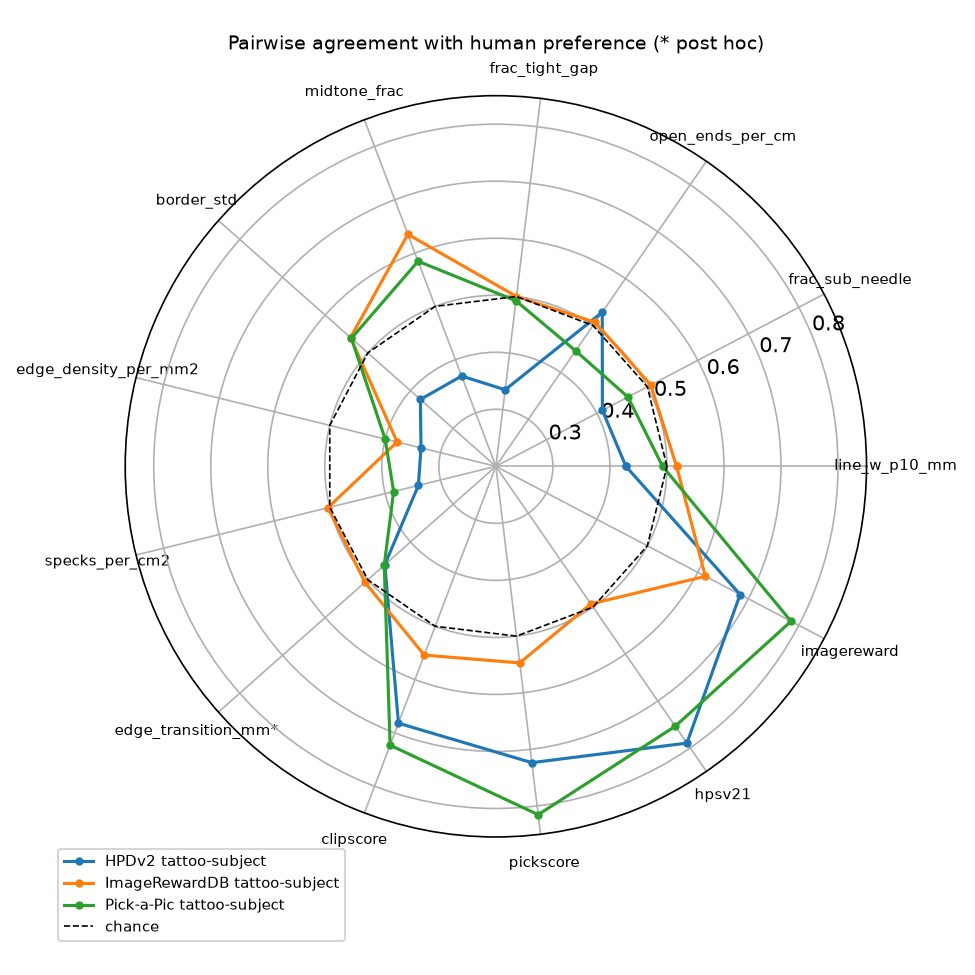
\includegraphics[width=0.48\linewidth]{figures/radar_per_dimension.png}
  \caption{Per-dimension agreement with human preference on the three tattoo-subject slices. Each spoke is one scorer. This is the same comparison as Table~\ref{tab:agree}, without the deprecated composite.}
  \label{fig:radar}
\end{figure}

% auto-generated by tables/make_tables.py
\begin{table}[t]
\centering
\caption{Pairwise accuracy $A$ against human preference on tattoo-subject pairs, the effect $A-0.5$, and Cohen's $h$ against $0.5$. The resampling unit is the prompt (cluster bootstrap, 2000 resamples, seed 0). $p_{\mathrm{Holm}}$ is a two-sided bootstrap $p$ after Holm correction within each dataset across all \NHpdTests\ scorers (the same count on each set: \NIrTests\ and \NPapTests). A printed floor means $p_{\mathrm{Holm}}\le$ that value, which is the bootstrap resolution. Holm-significant scorers: \NHpdSigholm/\NHpdTests\ on HPDv2, \NIrSigholm/\NIrTests\ on ImageRewardDB, \NPapSigholm/\NPapTests\ on Pick-a-Pic. Pair counts are \HpdHpstwoN, \IrHpstwoN\ and \PapHpstwoN. Edge transition is post hoc. HPSv2.1$\leftarrow$HPDv2, ImageReward$\leftarrow$ImageRewardDB and PickScore$\leftarrow$Pick-a-Pic v1 are in-distribution.}
\label{tab:agree}
\resizebox{\linewidth}{!}{%
\footnotesize
\begin{tabular}{lcccccccccccc}
\toprule
& \multicolumn{4}{c}{HPDv2} & \multicolumn{4}{c}{ImageRewardDB} & \multicolumn{4}{c}{Pick-a-Pic} \\
\cmidrule(lr){2-5}\cmidrule(lr){6-9}\cmidrule(lr){10-13}
Scorer & $A$ & $A{-}0.5$ & $h$ & $p_{\mathrm{Holm}}$ & $A$ & $A{-}0.5$ & $h$ & $p_{\mathrm{Holm}}$ & $A$ & $A{-}0.5$ & $h$ & $p_{\mathrm{Holm}}$ \\
\midrule
line\_w p10 & \HpdLinewpmmfiveAcc & \HpdLinewpmmfiveEffect & \HpdLinewpmmfiveH & \HpdLinewpmmfivePholm & \IrLinewpmmfiveAcc & \IrLinewpmmfiveEffect & \IrLinewpmmfiveH & \IrLinewpmmfivePholm & \PapLinewpmmfiveAcc & \PapLinewpmmfiveEffect & \PapLinewpmmfiveH & \PapLinewpmmfivePholm \\
frac sub-needle & \HpdFracsubneedlefiveAcc & \HpdFracsubneedlefiveEffect & \HpdFracsubneedlefiveH & \HpdFracsubneedlefivePholm & \IrFracsubneedlefiveAcc & \IrFracsubneedlefiveEffect & \IrFracsubneedlefiveH & \IrFracsubneedlefivePholm & \PapFracsubneedlefiveAcc & \PapFracsubneedlefiveEffect & \PapFracsubneedlefiveH & \PapFracsubneedlefivePholm \\
open ends / cm & \HpdOpenendspercmfiveAcc & \HpdOpenendspercmfiveEffect & \HpdOpenendspercmfiveH & \HpdOpenendspercmfivePholm & \IrOpenendspercmfiveAcc & \IrOpenendspercmfiveEffect & \IrOpenendspercmfiveH & \IrOpenendspercmfivePholm & \PapOpenendspercmfiveAcc & \PapOpenendspercmfiveEffect & \PapOpenendspercmfiveH & \PapOpenendspercmfivePholm \\
frac tight gap & \HpdFractightgapfiveAcc & \HpdFractightgapfiveEffect & \HpdFractightgapfiveH & \HpdFractightgapfivePholm & \IrFractightgapfiveAcc & \IrFractightgapfiveEffect & \IrFractightgapfiveH & \IrFractightgapfivePholm & \PapFractightgapfiveAcc & \PapFractightgapfiveEffect & \PapFractightgapfiveH & \PapFractightgapfivePholm \\
mid-tone frac. & \HpdMidtonefracfiveAcc & \HpdMidtonefracfiveEffect & \HpdMidtonefracfiveH & \HpdMidtonefracfivePholm & \IrMidtonefracfiveAcc & \IrMidtonefracfiveEffect & \IrMidtonefracfiveH & \IrMidtonefracfivePholm & \PapMidtonefracfiveAcc & \PapMidtonefracfiveEffect & \PapMidtonefracfiveH & \PapMidtonefracfivePholm \\
border std & \HpdBorderstdfiveAcc & \HpdBorderstdfiveEffect & \HpdBorderstdfiveH & \HpdBorderstdfivePholm & \IrBorderstdfiveAcc & \IrBorderstdfiveEffect & \IrBorderstdfiveH & \IrBorderstdfivePholm & \PapBorderstdfiveAcc & \PapBorderstdfiveEffect & \PapBorderstdfiveH & \PapBorderstdfivePholm \\
edge density & \HpdEdgedensitypermmfiveAcc & \HpdEdgedensitypermmfiveEffect & \HpdEdgedensitypermmfiveH & \HpdEdgedensitypermmfivePholm & \IrEdgedensitypermmfiveAcc & \IrEdgedensitypermmfiveEffect & \IrEdgedensitypermmfiveH & \IrEdgedensitypermmfivePholm & \PapEdgedensitypermmfiveAcc & \PapEdgedensitypermmfiveEffect & \PapEdgedensitypermmfiveH & \PapEdgedensitypermmfivePholm \\
specks / cm$^2$ & \HpdSpeckspercmfiveAcc & \HpdSpeckspercmfiveEffect & \HpdSpeckspercmfiveH & \HpdSpeckspercmfivePholm & \IrSpeckspercmfiveAcc & \IrSpeckspercmfiveEffect & \IrSpeckspercmfiveH & \IrSpeckspercmfivePholm & \PapSpeckspercmfiveAcc & \PapSpeckspercmfiveEffect & \PapSpeckspercmfiveH & \PapSpeckspercmfivePholm \\
edge transition & \HpdEdgetransitionmmfiveAcc & \HpdEdgetransitionmmfiveEffect & \HpdEdgetransitionmmfiveH & \HpdEdgetransitionmmfivePholm & \IrEdgetransitionmmfiveAcc & \IrEdgetransitionmmfiveEffect & \IrEdgetransitionmmfiveH & \IrEdgetransitionmmfivePholm & \PapEdgetransitionmmfiveAcc & \PapEdgetransitionmmfiveEffect & \PapEdgetransitionmmfiveH & \PapEdgetransitionmmfivePholm \\
CLIPScore & \HpdClipscoreAcc & \HpdClipscoreEffect & \HpdClipscoreH & \HpdClipscorePholm & \IrClipscoreAcc & \IrClipscoreEffect & \IrClipscoreH & \IrClipscorePholm & \PapClipscoreAcc & \PapClipscoreEffect & \PapClipscoreH & \PapClipscorePholm \\
PickScore & \HpdPickscoreAcc & \HpdPickscoreEffect & \HpdPickscoreH & \HpdPickscorePholm & \IrPickscoreAcc & \IrPickscoreEffect & \IrPickscoreH & \IrPickscorePholm & \PapPickscoreAcc & \PapPickscoreEffect & \PapPickscoreH & \PapPickscorePholm \\
HPSv2.1 & \HpdHpstwoAcc & \HpdHpstwoEffect & \HpdHpstwoH & \HpdHpstwoPholm & \IrHpstwoAcc & \IrHpstwoEffect & \IrHpstwoH & \IrHpstwoPholm & \PapHpstwoAcc & \PapHpstwoEffect & \PapHpstwoH & \PapHpstwoPholm \\
ImageReward & \HpdImagerewardAcc & \HpdImagerewardEffect & \HpdImagerewardH & \HpdImagerewardPholm & \IrImagerewardAcc & \IrImagerewardEffect & \IrImagerewardH & \IrImagerewardPholm & \PapImagerewardAcc & \PapImagerewardEffect & \PapImagerewardH & \PapImagerewardPholm \\
\bottomrule
\end{tabular}}
\end{table}


\subsection{Fusion learns the opposite signs}
A prompt-held-out logistic fusion of the eight pre-registered probes reaches \FusHpdProbespreregisteredAcc\ on HPDv2 (\FusHpdProbespreregisteredLo\ to \FusHpdProbespreregisteredHi, $n{=}\FusHpdProbespreregisteredN$).
Adding edge transition leaves \FusHpdProbesallAcc.
The full-sample coefficients invert the a-priori signs for line width, sub-needle fraction, tight gaps, mid-tones, border variation, edge density and specks.
Only open ends stay negative.
The fusion predicts annotator taste by rewarding features the probes call worse to tattoo.
Reward fusion reaches \FusHpdRewardsAcc\ ($n{=}\FusHpdRewardsN$) and is not improved by adding probes (\FusHpdRewardsprobesAcc).
In the reward-only fit the HPSv2.1 coefficient is positive and dominates; PickScore's coefficient is negative.

On ImageRewardDB the pre-registered probe fusion is \FusIrProbespreregisteredAcc\ (\FusIrProbespreregisteredLo\ to \FusIrProbespreregisteredHi).
Reward fusion is \FusIrRewardsAcc; adding probes lowers it to \FusIrRewardsprobesAcc.
The reward-only fit puts a positive sign on ImageReward and a negative sign on HPSv2.1.
We do not treat the probe signs on \NIrTsprompts\ prompts as stable.

On Pick-a-Pic the pre-registered probe fusion is \FusPapProbespreregisteredAcc\ (\FusPapProbespreregisteredLo\ to \FusPapProbespreregisteredHi, $n{=}\FusPapProbespreregisteredN$), below one half, and the all-probe fusion is \FusPapProbesallAcc.
The full-sample signs are not the HPDv2 inversion.
Line width is negative, and edge density and specks are positive, so those three disagree with the a-priori tattooability signs.
Sub-needle fraction, open ends, tight gaps, mid-tones and border variation keep the a-priori sign.
Reward fusion reaches \FusPapRewardsAcc\ (\FusPapRewardsLo\ to \FusPapRewardsHi); adding probes lowers it to \FusPapRewardsprobesAcc.
In the reward-only fit PickScore and ImageReward are positive and HPSv2.1 is negative.
The PickScore term is the leaky one.

% auto-generated by tables/make_tables.py
\begin{table}[t]
\centering
\caption{Prompt-held-out logistic fusion (GroupKFold on prompt, $k{=}5$, seed 0). Accuracy is the fraction of pairs whose held-out predicted winner matches the human winner. Brackets are 95\% prompt-cluster bootstrap intervals (2000 resamples). Coefficient signs are discussed in the text; magnitudes stay in \texttt{fusion\_lopo.csv}. On Pick-a-Pic the reward fusion is led by PickScore, which was trained on Pick-a-Pic v1.}
\label{tab:fusion}
\resizebox{\linewidth}{!}{%
\footnotesize
\begin{tabular}{lcccccc}
\toprule
Model & HPDv2 acc. [CI] & $n$ & ImageRewardDB acc. [CI] & $n$ & Pick-a-Pic acc. [CI] & $n$ \\
\midrule
Probes, pre-registered & \FusHpdProbespreregisteredAcc\ [\FusHpdProbespreregisteredLo, \FusHpdProbespreregisteredHi] & \FusHpdProbespreregisteredN & \FusIrProbespreregisteredAcc\ [\FusIrProbespreregisteredLo, \FusIrProbespreregisteredHi] & \FusIrProbespreregisteredN & \FusPapProbespreregisteredAcc\ [\FusPapProbespreregisteredLo, \FusPapProbespreregisteredHi] & \FusPapProbespreregisteredN \\
Probes, including edge transition & \FusHpdProbesallAcc\ [\FusHpdProbesallLo, \FusHpdProbesallHi] & \FusHpdProbesallN & \FusIrProbesallAcc\ [\FusIrProbesallLo, \FusIrProbesallHi] & \FusIrProbesallN & \FusPapProbesallAcc\ [\FusPapProbesallLo, \FusPapProbesallHi] & \FusPapProbesallN \\
Rewards & \FusHpdRewardsAcc\ [\FusHpdRewardsLo, \FusHpdRewardsHi] & \FusHpdRewardsN & \FusIrRewardsAcc\ [\FusIrRewardsLo, \FusIrRewardsHi] & \FusIrRewardsN & \FusPapRewardsAcc\ [\FusPapRewardsLo, \FusPapRewardsHi] & \FusPapRewardsN \\
Rewards + all probes & \FusHpdRewardsprobesAcc\ [\FusHpdRewardsprobesLo, \FusHpdRewardsprobesHi] & \FusHpdRewardsprobesN & \FusIrRewardsprobesAcc\ [\FusIrRewardsprobesLo, \FusIrRewardsprobesHi] & \FusIrRewardsprobesN & \FusPapRewardsprobesAcc\ [\FusPapRewardsprobesLo, \FusPapRewardsprobesHi] & \FusPapRewardsprobesN \\
\bottomrule
\end{tabular}}
\end{table}


\subsection{Injected defects}
Table~\ref{tab:degr} asks whether a known damage lowers the score.
At 5\,cm, edge transition rates blur at \DgEdgetransitionmmfiveBlurOne\ and \DgEdgetransitionmmfiveBlurTwo, detail loss at \DgEdgetransitionmmfiveDetaillossOne\ and \DgEdgetransitionmmfiveDetaillossTwo, and thickening at \DgEdgetransitionmmfiveThickenOne\ and \DgEdgetransitionmmfiveThickenTwo.
Mid-tone fraction rates haze at \DgMidtonefracfiveHazeOne\ and speckle at \DgMidtonefracfiveSpeckleOne.
Sub-needle fraction rates thinning at \DgFracsubneedlefiveThinOne\ and \DgFracsubneedlefiveThinTwo.
The deprecated composite is omitted here and stated once in Appendix~\ref{app:probes}.

HPSv2.1's lowest cell in the table is light blur at \DgHpstwoBlurOne.
PickScore on that cell is \DgPickscoreBlurOne.
CLIPScore on speckle is \DgClipscoreSpeckleOne\ and \DgClipscoreSpeckleTwo.
ImageReward on heavy speckle is \DgImagerewardSpeckleTwo.
Rewards detect many defects and do not name the millimetre quantity that moved.
Figure~\ref{fig:degr} shows the grid.

% auto-generated by tables/make_tables.py
\begin{table}[t]
\centering
\caption{Controlled-defect detection at a 5\,cm print size: fraction of designs on which the clean image scores better than the degraded image (ties count as one half). Probe columns use a-priori signs. Reward columns use the raw reward (higher is better). The deprecated composite is not a column here; Appendix~\ref{app:probes} states it in one sentence. $n{=}\nDegrRewDesigns$ designs per cell (the reward subset).}
\label{tab:degr}
\resizebox{\linewidth}{!}{%
\footnotesize
\begin{tabular}{llcccccccc}
\toprule
Defect & Lv. & trans. & sub-ndl & gap & mid & HPS & IR & Pick & CLIP \\
\midrule
blur & 1 & \DgEdgetransitionmmfiveBlurOne & \DgFracsubneedlefiveBlurOne & \DgFractightgapfiveBlurOne & \DgMidtonefracfiveBlurOne & \DgHpstwoBlurOne & \DgImagerewardBlurOne & \DgPickscoreBlurOne & \DgClipscoreBlurOne \\
blur & 2 & \DgEdgetransitionmmfiveBlurTwo & \DgFracsubneedlefiveBlurTwo & \DgFractightgapfiveBlurTwo & \DgMidtonefracfiveBlurTwo & \DgHpstwoBlurTwo & \DgImagerewardBlurTwo & \DgPickscoreBlurTwo & \DgClipscoreBlurTwo \\
detail loss & 1 & \DgEdgetransitionmmfiveDetaillossOne & \DgFracsubneedlefiveDetaillossOne & \DgFractightgapfiveDetaillossOne & \DgMidtonefracfiveDetaillossOne & \DgHpstwoDetaillossOne & \DgImagerewardDetaillossOne & \DgPickscoreDetaillossOne & \DgClipscoreDetaillossOne \\
detail loss & 2 & \DgEdgetransitionmmfiveDetaillossTwo & \DgFracsubneedlefiveDetaillossTwo & \DgFractightgapfiveDetaillossTwo & \DgMidtonefracfiveDetaillossTwo & \DgHpstwoDetaillossTwo & \DgImagerewardDetaillossTwo & \DgPickscoreDetaillossTwo & \DgClipscoreDetaillossTwo \\
haze & 1 & \DgEdgetransitionmmfiveHazeOne & \DgFracsubneedlefiveHazeOne & \DgFractightgapfiveHazeOne & \DgMidtonefracfiveHazeOne & \DgHpstwoHazeOne & \DgImagerewardHazeOne & \DgPickscoreHazeOne & \DgClipscoreHazeOne \\
haze & 2 & \DgEdgetransitionmmfiveHazeTwo & \DgFracsubneedlefiveHazeTwo & \DgFractightgapfiveHazeTwo & \DgMidtonefracfiveHazeTwo & \DgHpstwoHazeTwo & \DgImagerewardHazeTwo & \DgPickscoreHazeTwo & \DgClipscoreHazeTwo \\
speckle & 1 & \DgEdgetransitionmmfiveSpeckleOne & \DgFracsubneedlefiveSpeckleOne & \DgFractightgapfiveSpeckleOne & \DgMidtonefracfiveSpeckleOne & \DgHpstwoSpeckleOne & \DgImagerewardSpeckleOne & \DgPickscoreSpeckleOne & \DgClipscoreSpeckleOne \\
speckle & 2 & \DgEdgetransitionmmfiveSpeckleTwo & \DgFracsubneedlefiveSpeckleTwo & \DgFractightgapfiveSpeckleTwo & \DgMidtonefracfiveSpeckleTwo & \DgHpstwoSpeckleTwo & \DgImagerewardSpeckleTwo & \DgPickscoreSpeckleTwo & \DgClipscoreSpeckleTwo \\
thicken & 1 & \DgEdgetransitionmmfiveThickenOne & \DgFracsubneedlefiveThickenOne & \DgFractightgapfiveThickenOne & \DgMidtonefracfiveThickenOne & \DgHpstwoThickenOne & \DgImagerewardThickenOne & \DgPickscoreThickenOne & \DgClipscoreThickenOne \\
thicken & 2 & \DgEdgetransitionmmfiveThickenTwo & \DgFracsubneedlefiveThickenTwo & \DgFractightgapfiveThickenTwo & \DgMidtonefracfiveThickenTwo & \DgHpstwoThickenTwo & \DgImagerewardThickenTwo & \DgPickscoreThickenTwo & \DgClipscoreThickenTwo \\
thin & 1 & \DgEdgetransitionmmfiveThinOne & \DgFracsubneedlefiveThinOne & \DgFractightgapfiveThinOne & \DgMidtonefracfiveThinOne & \DgHpstwoThinOne & \DgImagerewardThinOne & \DgPickscoreThinOne & \DgClipscoreThinOne \\
thin & 2 & \DgEdgetransitionmmfiveThinTwo & \DgFracsubneedlefiveThinTwo & \DgFractightgapfiveThinTwo & \DgMidtonefracfiveThinTwo & \DgHpstwoThinTwo & \DgImagerewardThinTwo & \DgPickscoreThinTwo & \DgClipscoreThinTwo \\
\bottomrule
\end{tabular}}
\end{table}


\begin{figure}[htbp]
  \centering
  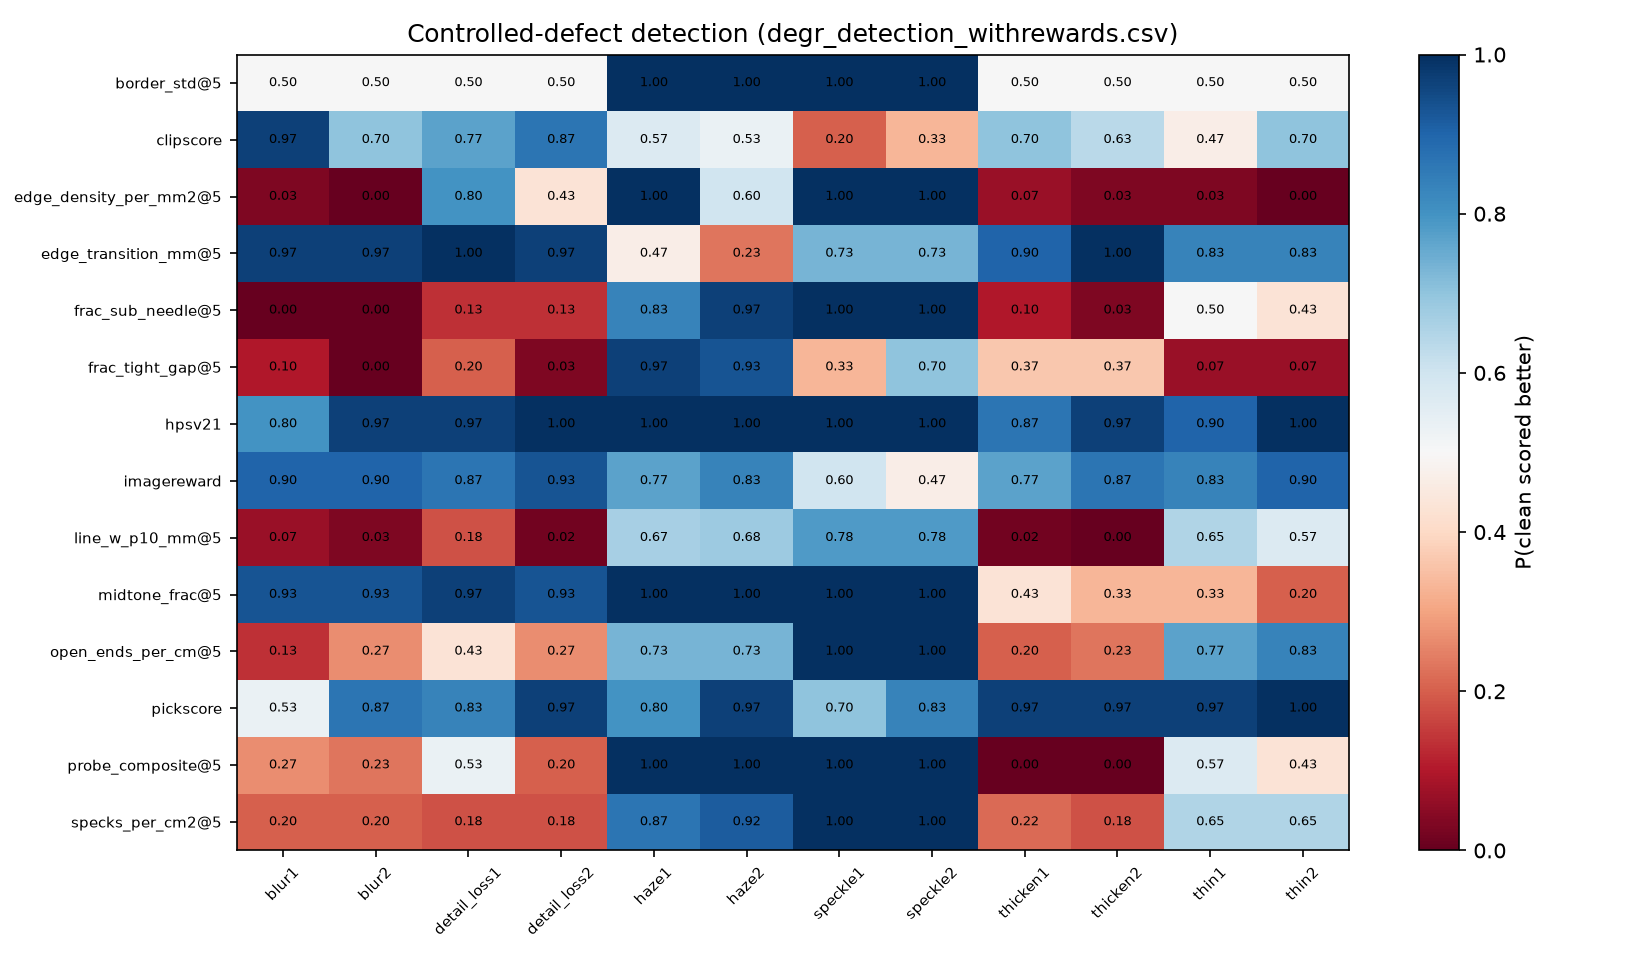
\includegraphics[width=0.55\linewidth]{figures/degr_detection.png}
  \caption{Detection rates on six injected defects at two strengths. The 5\,cm numbers for the probes we interpret, and for the four rewards, are in Table~\ref{tab:degr}.}
  \label{fig:degr}
\end{figure}

\subsection{Scale and spread}
With no additive pixel noise, skeleton $F_1$ at spread $\sigma{=}0$ is \ssFoneSizeThreeSpreadZero\ at $s{=}3$\,cm, \ssFoneSizeFiveSpreadZero\ at $s{=}5$\,cm, \ssFoneSizeTenSpreadZero\ at $s{=}10$\,cm and \ssFoneSizeFifteenSpreadZero\ at $s{=}15$\,cm (Table~\ref{tab:scale}, Figure~\ref{fig:scale}).
The same four sizes under the old $\sigma{=}4$ grey-level noise are \ssNoiseFoneThree, \ssNoiseFoneFive, \ssNoiseFoneTen\ and \ssNoiseFoneFifteen, which fall as the print grows.
That fall is not in the default grid.
At 0.30\,mm spread, default $F_1$ is \ssFoneSizeThreeSpreadThirty, \ssFoneSizeFiveSpreadThirty, \ssFoneSizeTenSpreadThirty\ and \ssFoneSizeFifteenSpreadThirty.
At 0.60\,mm it is \ssFoneSizeThreeSpreadSixty, \ssFoneSizeFiveSpreadSixty, \ssFoneSizeTenSpreadSixty\ and \ssFoneSizeFifteenSpreadSixty.
Gap survival at 0.30\,mm is \ssGapSizeThreeSpreadThirty, \ssGapSizeFiveSpreadThirty, \ssGapSizeTenSpreadThirty\ and \ssGapSizeFifteenSpreadThirty.
Table~\ref{tab:scale} reports a subset of that 0.05\,mm grid.

Table~\ref{tab:minsize} is the size at which mean skeleton $F_1$ first reaches seven tenths, and eight tenths.
At zero spread both levels are met at \minSizeSeventySpreadZero\,cm.
At 0.20\,mm the seven-tenths size is \minSizeSeventySpreadTwenty\,cm and the eight-tenths size is \minSizeEightySpreadTwenty\,cm.
At 0.30\,mm the seven-tenths size is \minSizeSeventySpreadThirty\,cm and eight tenths is \minSizeEightySpreadThirty.
At 0.60\,mm neither level is reached (\minSizeSeventySpreadSixty, \minSizeEightySpreadSixty).

At 5\,cm and 0.30\,mm, tight-gap fraction correlates with gap survival at \RhoFractightgapGapsurvival\ (partly circular), edge density with gap survival at \RhoEdgedensitypermmGapsurvival, edge transition with skeleton $F_1$ at \RhoEdgetransitionmmSkelf, and minimum line width with skeleton $F_1$ at \RhoLinewpmmSkelf.
These associations live inside the simulator.

\begin{figure}[htbp]
  \centering
  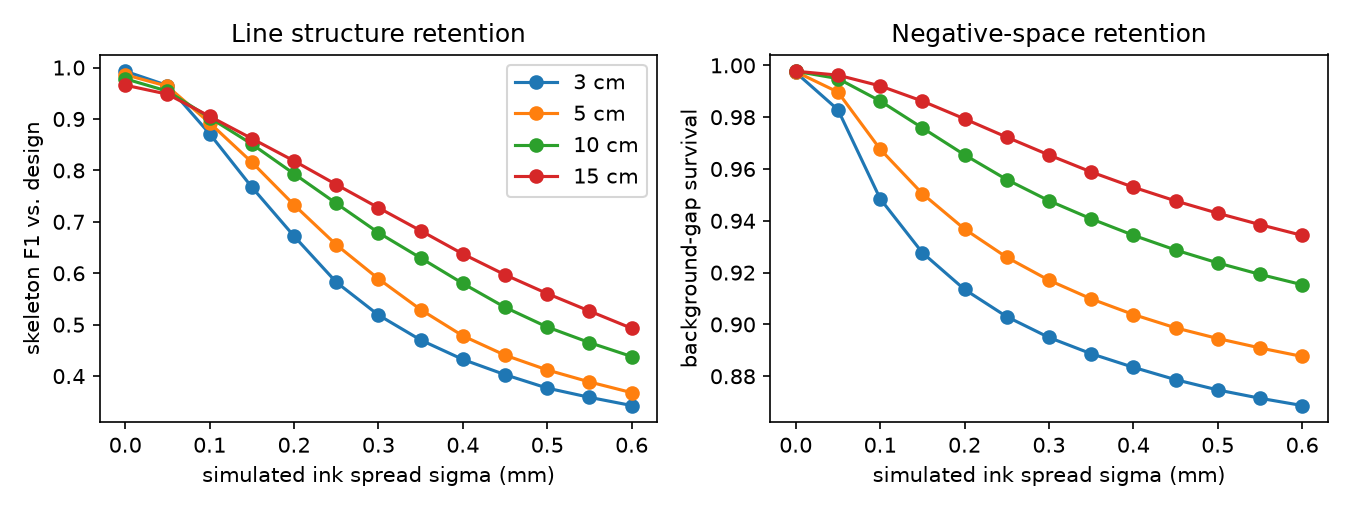
\includegraphics[width=0.72\linewidth]{figures/scale_spread.png}
  \caption{Mean skeleton $F_1$ against ink spread $\sigma$ at each print size $s$. The grid is the default simulator: no additive pixel noise. Table~\ref{tab:scale} lists a subset of the same cells.}
  \label{fig:scale}
\end{figure}

% auto-generated by tables/make_tables.py
\begin{table}[t]
\centering
\caption{Mean skeleton $F_1$ (tolerance 0.2\,mm) and, on the following row, mean gap survival. Default simulation: no additive pixel noise, and the same Otsu threshold on the reference and the blurred image. Rows are longest-side print sizes in centimetres. Columns are a subset of the 0 to 0.60\,mm grid (step 0.05\,mm); the figure shows every step. Each cell averages \nDegrDesigns\ designs. At spread 0, $F_1$ is exact on this grid.}
\label{tab:scale}
\resizebox{\linewidth}{!}{%
\footnotesize
\begin{tabular}{lccccc}
\toprule
Size (cm) & 0 & 0.15 & 0.30 & 0.45 & 0.60 \\
\midrule
3 & \ssFoneSizeThreeSpreadZero & \ssFoneSizeThreeSpreadFifteen & \ssFoneSizeThreeSpreadThirty & \ssFoneSizeThreeSpreadFortyFive & \ssFoneSizeThreeSpreadSixty \\
3 (gap) & \ssGapSizeThreeSpreadZero & \ssGapSizeThreeSpreadFifteen & \ssGapSizeThreeSpreadThirty & \ssGapSizeThreeSpreadFortyFive & \ssGapSizeThreeSpreadSixty \\
5 & \ssFoneSizeFiveSpreadZero & \ssFoneSizeFiveSpreadFifteen & \ssFoneSizeFiveSpreadThirty & \ssFoneSizeFiveSpreadFortyFive & \ssFoneSizeFiveSpreadSixty \\
5 (gap) & \ssGapSizeFiveSpreadZero & \ssGapSizeFiveSpreadFifteen & \ssGapSizeFiveSpreadThirty & \ssGapSizeFiveSpreadFortyFive & \ssGapSizeFiveSpreadSixty \\
10 & \ssFoneSizeTenSpreadZero & \ssFoneSizeTenSpreadFifteen & \ssFoneSizeTenSpreadThirty & \ssFoneSizeTenSpreadFortyFive & \ssFoneSizeTenSpreadSixty \\
10 (gap) & \ssGapSizeTenSpreadZero & \ssGapSizeTenSpreadFifteen & \ssGapSizeTenSpreadThirty & \ssGapSizeTenSpreadFortyFive & \ssGapSizeTenSpreadSixty \\
15 & \ssFoneSizeFifteenSpreadZero & \ssFoneSizeFifteenSpreadFifteen & \ssFoneSizeFifteenSpreadThirty & \ssFoneSizeFifteenSpreadFortyFive & \ssFoneSizeFifteenSpreadSixty \\
15 (gap) & \ssGapSizeFifteenSpreadZero & \ssGapSizeFifteenSpreadFifteen & \ssGapSizeFifteenSpreadThirty & \ssGapSizeFifteenSpreadFortyFive & \ssGapSizeFifteenSpreadSixty \\
\bottomrule
\end{tabular}}
\end{table}

% auto-generated by tables/make_tables.py
\begin{table}[t]
\centering
\caption{Smallest tested print size, in centimetres, whose mean skeleton $F_1$ reaches seven tenths or eight tenths at that spread. \texttt{n/a} means no tested size up to 15\,cm reached the level. Noise is off. This is a sensitivity table for the simulator, not a healed-skin recommendation.}
\label{tab:minsize}
\footnotesize
\begin{tabular}{lcc}
\toprule
Spread (mm) & Min.\ size, $F_1$ seven tenths & Min.\ size, $F_1$ eight tenths \\
\midrule
0 & \minSizeSeventySpreadZero & \minSizeEightySpreadZero \\
0.10 & \minSizeSeventySpreadTen & \minSizeEightySpreadTen \\
0.20 & \minSizeSeventySpreadTwenty & \minSizeEightySpreadTwenty \\
0.30 & \minSizeSeventySpreadThirty & \minSizeEightySpreadThirty \\
0.40 & \minSizeSeventySpreadForty & \minSizeEightySpreadForty \\
0.50 & \minSizeSeventySpreadFifty & \minSizeEightySpreadFifty \\
0.60 & \minSizeSeventySpreadSixty & \minSizeEightySpreadSixty \\
\bottomrule
\end{tabular}
\end{table}




\section{Discussion}
\label{sec:discussion}

The preference result and the defect result answer different questions, and they should not be averaged into one leaderboard.

On HPDv2 tattoo-subject pairs, human winners are the images our a-priori probes call worse to tattoo.
Dense shading, tight spacing and thin lines are attractive on a screen.
They are also the features a needle of width $w_n$ and a gap of width $g$ penalise.
A prompt-held-out fusion can predict the annotator, at \FusHpdProbespreregisteredAcc, only by flipping those penalties.
Using that fusion as a tattooability reward would optimise the opposite of the probe specification.
Using HPSv2.1 as a tattooability reward would do the same thing for a different reason: it agrees with the annotators (\HpdHpstwoAcc) on data it was trained on, and it has no millimetre scale.

Edge transition separates blur, detail loss and thickening from the clean image.
Mid-tone fraction separates haze and speckle.
Sub-needle fraction separates thinning.
The deprecated composite cancels some of those effects because thickening improves a width probe while hurting a gap probe.
Per-dimension reporting is the property the reward models do not have: HPSv2.1 detects most injected defects and does not name which geometric fact changed.

The Pick-a-Pic tattoo-subject slice is only \PapHpstwoN\ pairs.
Probe fusion there stays below one half (\FusPapProbespreregisteredAcc) and does not reproduce the HPDv2 sign flip in full.
Reward fusion is high (\FusPapRewardsAcc) with a positive PickScore coefficient, which is training leakage from Pick-a-Pic v1, not a new external test.
HPSv2.1 and ImageReward were not trained on that set; their Pick-a-Pic intervals are still wide.

ImageRewardDB does not rescue a positive probe--preference correlation.
The point estimates sit near chance, the prompt count is \NIrTsprompts, and ImageReward's own accuracy on that set is an in-distribution number with a wide interval.
A claim that ``rewards ignore tattooability'' is too broad: several rewards notice blur, haze and thinning in the injection study.
The supported claim is narrower.
Preference on the public tattoo-subject pairs we could score is not a tattooability label, and models trained to imitate that preference should not be described as if it were.

\begin{figure}[htbp]
  \centering
  
\includegraphics[width=0.92\linewidth]{figures/tatany_illustrative.png}
  \caption{The author operates tatany.app.
  The images are tatany.app product case images (marketing mock-ups cropped to one panel; provenance in supplementary notes).
  Probes at $s{=}5$\,cm and a simulated spread $\sigma{=}0.20$\,mm are shown for illustration only.
  tatany is not ranked, evaluated or compared with any other system.}
  \label{fig:tatany}
\end{figure}

A practical screen for AI tattoo generation can reject sub-needle line mass, tight gaps and soft transitions at the intended print size $s$.
Those gates disagree with current preference rewards on the HPDv2 pairs above.
That disagreement is a reason to keep the gates.

\section{Limitations}
\label{sec:limitations}

Tattoo-subject prompt counts are small outside HPDv2.
ImageRewardDB contributes \NIrTsprompts\ prompts and Pick-a-Pic \NPapTsprompts.
Cluster-bootstrap intervals on those sets are wide, and after Holm no probe is significant (\NIrSigholm\ of \NIrTests\ scorers on ImageRewardDB; the single Pick-a-Pic rejection is PickScore, \NPapSigholm\ of \NPapTests).
Those rows do not support a model ranking.

The class filter mixes keywords, CLIP zero-shot, and a single non-blinded annotator on \nAmb\ ambiguous images.
A design-versus-portrait error changes which pairs enter Table~\ref{tab:agree}.

Needle width $w_n$ and gap width $g$ are practitioner-scale assumptions, not measurements from this study.
Other machines, other skin, and colour packing change both numbers.
The ink-spread simulator is an isotropic Gaussian at a stated $\sigma$.
It is unvalidated on healed skin.
Real ink does not spread as a circular blur, and we have no paired photograph of a design before and after healing.
With noise off, skeleton $F_1$ at $\sigma{=}0$ is \ssFoneSizeThreeSpreadZero\ at every tested size $s$, including 15\,cm (\ssFoneSizeFifteenSpreadZero).
The earlier decline with size was grey-level noise of pixel standard deviation 4, which leaves \ssNoiseFoneThree\ at $s{=}3$\,cm and \ssNoiseFoneFifteen\ at $s{=}15$\,cm.
Removing that artifact does not make the Gaussian a model of healed skin.
At 0.60\,mm spread, no tested size reaches mean $F_1$ of seven tenths (\minSizeSeventySpreadSixty).

Reward-model scores leak their training sets.
HPSv2.1 was trained on HPDv2, ImageReward on ImageRewardDB, and PickScore on Pick-a-Pic.
We cannot remove the tattoo-subject pairs from those training sets retroactively.
CLIPScore was not trained as a preference model.
The Pick-a-Pic licence is uncertain: the original dataset card has been removed, and mirrors say MIT.
We did not verify that statement.

Otsu thresholding and the greyscale conversion assume a dark-ink-on-light-paper drawing.
Colour work, skin photographs and mid-grey packing violate that assumption, and the probes still emit a number.
Edge-transition width is a post-hoc probe, chosen after the first controlled-degradation run.
Its preference accuracy is exploratory.
Defects are synthetic and one at a time, and reward detection uses \nDegrRewDesigns\ designs.
The composite mixes probes whose signs fight each other under thickening.
It is deprecated and is not a column of Table~\ref{tab:degr}.

Figure~\ref{fig:tatany} is a marketing mock-up.
The panels are tatany.app product case images, cropped to one panel, not logged generations.
Background paper and skin texture change what a probe would read, which is why the figure is illustration only and why per-image probe values are not quoted.
No commercial AI tattoo generator was ranked.
Generalising from HPDv2 to images produced by a product model would be a new study.

\section{Conclusion}
\label{sec:conclusion}

Preference is not tattooability on the pairs we audited.
On HPDv2 tattoo-subject pairs, pre-registered probes that penalise dense, shaded, thin-line images agree with human winners below chance.
The tight-gap probe, for example, agrees on \HpdFractightgapfiveAcc\ of pairs.
A prompt-held-out fusion of the probes reaches \FusHpdProbespreregisteredAcc\ by assigning the opposite signs.
HPSv2.1 agrees with those annotators at \HpdHpstwoAcc\ on data it was trained on.
ImageReward agrees with ImageRewardDB annotators at \IrImagerewardAcc, with a wide interval and only \NIrTsprompts\ tattoo-subject prompts.

The same probes, read one at a time, detect the injected defects they were defined for, and the reward models detect many of those defects too, without a physical unit.
A Pick-a-Pic slice of \PapHpstwoN\ pairs does not overturn the HPDv2 result, and PickScore on it is in-distribution.
A Gaussian scale-and-spread stress test, with no additive pixel noise, keeps skeleton $F_1$ at \ssFoneSizeThreeSpreadZero\ when the spread is $\sigma{=}0$ and lowers it as $\sigma$ grows.
It remains an assumption, not a skin study.

For AI tattoo generation, a preference reward is evidence about annotators.
A millimetre probe is evidence about a declared needle, gap and print size.
Reporting those probes separately, and stating when a reward model is scored in distribution, is the audit.

\section*{Resources and data availability}
Probe definitions, degradation operators and the analysis scripts live with the study code that produced \texttt{numbers.tex}.
HPDv2, ImageRewardDB and Pick-a-Pic are used under the terms of their public releases \citep{wu2023hpsv2,xu2023imagereward,kirstain2023pickapic}.
Drozdik/tattoo\_v0 is CC BY-NC-SA and was used for research only; we do not redistribute it.
Pick-a-Pic metadata and images were read locally from a mirror whose MIT statement we could not verify against the removed original card.
They are not redistributed.
Derived pair counts and scores are the tables in this paper.

\section*{Declaration of competing interest}
\label{sec:coi}
The author operates tatany.app, a commercial AI tattoo generator.
That conflict is relevant because a published critique of generic preference rewards could favour a product that advertises tattoo-specific checks.
tatany was not evaluated or ranked.
No tatany output appears in HPDv2, ImageRewardDB, Pick-a-Pic, the defect set, or the spread test.
The probes were not tuned on tatany images.

\section*{Acknowledgements}
We thank the maintainers of HPDv2, ImageRewardDB, Pick-a-Pic and Drozdik/tattoo\_v0 for releasing data.
The ambiguous-class review was done by the author's assistant, as a single non-blinded rater.


\appendix
\section{Probe implementation notes}
\label{app:probes}

Distance transforms use a $5{\times}5$ mask.
Skeleton endpoints are pixels whose $3{\times}3$ neighbour sum equals 2, and the open-end rate divides that count by skeleton length in centimetres.
Tight gaps use the background inside the ink box only.
Specks are 8-connected ink components smaller than $(0.30 \times 10)^2$ pixels.
Mid-tones lie strictly inside grey $(60, 200)$, the border band is 5\,px, and Canny hysteresis is 50 and 150 \citep{canny1986}.
Otsu is replaced by a fixed mid-grey cut when the grey standard deviation is at most 1 \citep{otsu1979}.
Thinning is Zhang--Suen \citep{zhang1984thinning}.
Edge transition divides median paper-minus-ink contrast by median Sobel magnitude on Canny pixels ($3{\times}3$ Sobel, one-eighth scale) and divides by 10\,px/mm.
Empty masks yield 0.
The deprecated composite is the mean of signed robust $z$-scores, using the median and interquartile range inside the scored pool.
On the defect subset it rates haze and speckle at \DgProbecompositefiveHazeOne\ and \DgProbecompositefiveSpeckleOne, thickening at \DgProbecompositefiveThickenOne\ and \DgProbecompositefiveThickenTwo, and light blur at \DgProbecompositefiveBlurOne.
Thickening moves the width term and the gap term in opposite directions, which is why that average is not a primary result.

The spread test blurs with $\sigma$ in millimetres times 10\,px/mm and, in the reported grid, adds no pixel noise.
Skeleton $F_1$ uses a square tolerance of width $2 \times \mathrm{round}(0.2 \times 10) + 1$ pixels.
The reference mask and the spread mask use one shared Otsu threshold.
SSIM is not computed \citep{wang2004ssim}.
Bootstrap, fusion, design sampling, speckle and haze noise use seed 0.

\section{Pre-registration record}
\label{app:prereg}

Phase-1 probes and signs, fixed before any preference accuracy was computed, are the eight quantities in Section~\ref{sec:method}: line width $+1$; sub-needle fraction, open ends, tight gaps, mid-tone fraction, border variation, edge density and specks all $-1$.
The primary estimand is pairwise accuracy on tattoo-subject pairs, with a 2000-resample prompt-cluster bootstrap and seed 0, at a 5\,cm print size, needle 0.30\,mm and gap 0.50\,mm.
The unweighted signed composite was defined in advance.
It is in Table~\ref{tab:degr} and is deprecated in favour of Table~\ref{tab:agree}.

\texttt{edge\_transition\_mm} (sign $-1$) was added after the first controlled-degradation run, which showed that blur and detail loss did not reliably shrink lines below 0.30\,mm or create specks.
Its detection rates are descriptive.
Its preference accuracies, \HpdEdgetransitionmmfiveAcc\ on HPDv2, \IrEdgetransitionmmfiveAcc\ on ImageRewardDB and \PapEdgetransitionmmfiveAcc\ on Pick-a-Pic, were not registered tests.
The pre-registered fusion excludes it.
The fusion that includes it does not change the conclusion.
Full-sample HPDv2 probe coefficients invert the registered signs for every pre-registered feature except open ends, which stay negative.
Those inverted signs are part of the negative result, not a specification we chose in advance.

Automatic labels left \NHpdClsAmbiguous\ HPDv2 images and \NIrClsAmbiguous\ ImageRewardDB images ambiguous, \nAmb\ images in total.
A single non-blinded rater, the author's assistant, assigned design (\NambDesign), on-skin (\NambOnskin), incidental (\NambIncidental) and other (\NambOther).
The rater saw the prompt and knew the labels would define the tattoo-subject subset.
This was not a blinded adjudication.
Counts after replacement are the ``after review'' rows of Table~\ref{tab:data}.

Pick-a-Pic scoring was added after the HPDv2 and ImageRewardDB runs.
Keyword selection yielded \nPAPkwPairs\ labelled pairs over \nPAPkwPrompts\ prompts; after CLIP filtering, \PapHpstwoN\ design or on-skin pairs over \NPapTsprompts\ prompts remain.
That analysis was not in the Phase-1 registration.
PickScore's accuracy on it is leaky because PickScore was trained on Pick-a-Pic v1.
The Gaussian grid is a sensitivity check, not a registered test on healed skin.
Its default has no additive pixel noise, so skeleton $F_1$ at spread 0 is \ssFoneSizeFiveSpreadZero\ at 5\,cm rather than the noise-on value \ssNoiseFoneFive.
Reward detection of injected defects uses \nDegrRewDesigns\ designs after a probe pass on \nDegrDesigns\ designs, and is not a registered superiority test.
Training overlap for HPSv2.1 and ImageReward was known from the dataset papers before scoring \citep{wu2023hpsv2,xu2023imagereward}.
A title-and-abstract search did not find a prior audit of preference rewards against millimetre tattoo probes.
Semantic Scholar and Google Scholar were not fully queried.

Spearman correlations at 5\,cm and 0.30\,mm spread, each over \nDegrDesigns\ designs, are in Table~\ref{tab:rho}.
The headline four are also stated in Section~\ref{sec:results}.

% auto-generated by tables/make_tables.py
\begin{table}[t]
\centering
\caption{Spearman rank correlation, at 5\,cm and 0.30\,mm spread, between a clean-image probe and the simulated outcome on that design ($n{=}\nDegrDesigns$). Gap survival versus tight-gap fraction is partly circular: both read narrow background gaps. These correlations are not a healed-skin validation.}
\label{tab:rho}
\footnotesize
\begin{tabular}{lcc}
\toprule
Probe on the clean design & $\rho$ vs.\ skeleton $F_1$ & $\rho$ vs.\ gap survival \\
\midrule
line\_w p10 & \RhoLinewpmmSkelf & \RhoLinewpmmGapsurvival \\
frac sub-needle & \RhoFracsubneedleSkelf & \RhoFracsubneedleGapsurvival \\
open ends & \RhoOpenendspercmSkelf & \RhoOpenendspercmGapsurvival \\
frac tight gap & \RhoFractightgapSkelf & \RhoFractightgapGapsurvival \\
mid-tone frac. & \RhoMidtonefracSkelf & \RhoMidtonefracGapsurvival \\
border std & \RhoBorderstdSkelf & \RhoBorderstdGapsurvival \\
edge transition & \RhoEdgetransitionmmSkelf & \RhoEdgetransitionmmGapsurvival \\
edge density & \RhoEdgedensitypermmSkelf & \RhoEdgedensitypermmGapsurvival \\
specks & \RhoSpeckspercmSkelf & \RhoSpeckspercmGapsurvival \\
ink fraction & \RhoInkfracSkelf & \RhoInkfracGapsurvival \\
\bottomrule
\end{tabular}
\end{table}

\enlargethispage{2\baselineskip}


\begingroup
\footnotesize
\bibliographystyle{unsrtnat}
\emergencystretch=2em
\bibliography{refs}
\endgroup

\end{document}
